\documentclass[letterpaper, openright, 12pt]{book}
\usepackage[spanish]{babel}
\usepackage[utf8]{inputenc}

\usepackage{graphicx} % para imagenes
\usepackage{subfigure} % para subfiguras
\usepackage{caption}

\usepackage{physics} % para formulas matemáticas
\usepackage{amsmath}

\usepackage[left=2cm,top=2cm,right=2cm,bottom=2cm]{geometry} % controla márgenes
\usepackage{cite} % para dar formato a las referencias bibliográficas
\usepackage{enumerate} % para hacer listas
\usepackage[hidelinks]{hyperref}
\usepackage{cleveref}



% Cabiar el titulo por default de los indices
\addto{\captionsspanish}{\renewcommand*{\listfigurename}{Indice de Figuras}} %cambia el nombre del indice de figuras
\addto{\captionsspanish}{\renewcommand*{\contentsname}{Indice}} 
\addto{\captionsspanish}{\renewcommand*{\listtablename}{Indice de Tablas}}


\pagestyle{plain} %sin cabeceras en las páginas, numero de pagina centrado abajo
\begin{document}
	\begin{titlepage}
		\begin{center}
			\begin{figure}
				\begin{center}
					
\includegraphics[width=3cm]{./Imagenes/ipn-logo}
				\end{center}	
			\end{figure}
		\rule{100mm}{0.3mm}\\
		\vspace*{8mm}
		\textbf{INSTITUTO POLITÉCNICO NACIONAL}\\
		\vspace*{3mm}
		ESCUELA SUPERIOR DE INGENIERÍA MECÁNICA Y ELÉCTRICA\\
		UNIDAD PROFESIONAL TICOMÁN\\
		\vspace{12mm}
		\textbf{DESARROLLO DE PAQUETERÍA DE SOFTWARE OPEN SOURCE EN LENGUAJE PYTHON PARA LA GENERACIÓN DE MALLAS}\\
		\vspace*{12mm}
		TESIS\\
		Que para obtener el grado de\\
		\vspace{3mm}
		INGENIERO EN AERONÁUTICA\\
		\vspace{12mm}
		PRESENTA\\
		\vspace{3mm}
		MARCO ANTONIO CARDOSO MORENO\\
		\rule{100mm}{0.3mm}\\
		\vspace{3mm}
		DIRECTOR DE TESIS: M. {\scriptsize EN} C. RAFAEL MEDINA NOGUERÓN
		\end{center}
	\vspace{6cm}
	\begin{flushleft}
		Ciudad de México
	\end{flushleft}
	\end{titlepage}
	%
	%
	%
	%
	%
	
	%
	%
	%
	%
	%
	\newpage\
	\thispagestyle{empty}
	%se deja hoja en blanco
	%
	%
	%
	%
	%
	
	%
	%
	%
	%
	% Dedicatoria
	\newpage
	\pagenumbering{Roman}
	\begin{flushright}
		\textit{Dedicado a Floresauria Fulgencia, amor de mi vida!}
	\end{flushright}
	\ % final página dedicatorias
	%
	%
	%
	%
	%
	
	%
	%
	%
	%
	%
	\chapter*{Agradecimientos}
	%
	%
	%
	%
	%
	
	%
	%
	%
	%
	%
	\chapter*{Resúmen}
	%
	%
	%
	%
	%
	
	%
	%
	%
	%
	% indices
	\tableofcontents
	
	\cleardoublepage
	\phantomsection % corrige error de hipervinculos que manda a la seccion previa
	\addcontentsline{toc}{chapter}{Indice de Figuras}
	\listoffigures
	
	
	\cleardoublepage
	\phantomsection % corrige error de hipervinculos que manda a la seccion previa
	\addcontentsline{toc}{chapter}{Indice de Tablas}
	\listoftables
	\cleardoublepage
	%
	%
	%
	%
	%
	
	%
	%
	%
	%
	%
	\chapter*{Nomenclatura}
	\addcontentsline{toc}{chapter}{Nomenclatura} % para agregar al índice
	%
	%
	%
	%
	%
	
	%
	%
	%
	%
	%
	\chapter*{Introducción}
	\addcontentsline{toc}{chapter}{Introducción}
	\paragraph*{}
		En general, para analizar y diseñar sistemas en los cuales interviene el flujo de fluidos se cuenta con dos herramientas: la experimentación y el cálculo. La experimentación implica la construcción de modelos que serán probados en túneles de viento u otras instalaciones. En el caso del cálculo, se puede realizar de manera analítica o mediante el uso de métodos númericos, a esta última técnica se le da el nombre de dinamica de fluidos computacional (CFD, por sus siglas en inglés). El uso de la DFC (dinámica de fluidos computacional) se ha popularizado gracias al desarrollo de las capaciades de las computadoras, ya que las simulaciones presentan ciertas ventajas frente al enfoque exprimental en términos de velocidad, seguridad y en la mayoría de casos, de costo. Gracias a esto la DFC es ampliamente usada en la actualidad en sectores de la industria como el aeroespacial, petrolero, entre otros. En el ámbito de la investigación tambien se tiene en la DFC una herramienta importante, pues permite analizar fenomenos complejos que pueden resultar dificiles de reproducir en experimentos.
	
	\paragraph*{}
		Se realiza el presente trabajo con la finalidad tanto de generar en los estudiantes un interés por la dinámica de fluidos computacional (CFD), como de fomentar el desarrollo de este campo mediante la implementación de códigos. Por otro lado, se busca fomentar en el lector el uso y desarrollo de software libre.

	\paragraph*{}
		En el capítulo 1....\\************añadir descripción breve de los capítulos****************




	\chapter*{Objetivo}
	\addcontentsline{toc}{chapter}{Objetivo}
	
	\paragraph*{}
	Desarrollar códigos que sean capaces de generar mallas mediante diferentes métodos. Dichos códigos se implementarán en lenguaje Python 3, mediante la IDE (entorno de desarrollo integrado, por sus siglas en inglés) Spyder, la cual fue creada pensando específicamente en la implementación de códigos enfocados a aspectos científicos y numéricos, 	que además presenta una interfaz gráfica similar a la de Matlab u Octave.
		
	\paragraph*{}
		El programa debe ser capaz de generar  mallas mediantes diferentes métodos, en este trabajo se presta principal atención a las mallas generadas por métodos algebráicos, así como por métodos basados en la solución de sistemas de ecuaciones diferenciales parciales, más específico, en EDP elípticas. Se debe generar la malla para cualquier superficie o forma deseada, en este trabajo se hace la generación de mallas alrededor de perfiles alares, por lo que se debe desarrollar un módulo que genere la nube de puntos que describe un perfil NACA de la serie 4, pudiendo ser ajustable la densidad de puntos de la misma. También se da la opción de importar la nube de puntos de cualquier otro perfil, con la restricción de que la densidad de la misma, depende de los datos de entrada que recibe el código.
	
	\paragraph*{}
		Una vez generado el mallado del dominio, se creará un archivo que contenga toda la información de la misma, el cual podrá ser importado a cualquier software \textit{``solver''}, para poder llevar a cabo el análisis de flujo deseado.



	
	\chapter*{Motivación}
	\addcontentsline{toc}{chapter}{Motivación}
	\paragraph*{}
		Existe en la actualidad, una vasta cantidad de software enfocado a la dinámica de fluidos computacional, tanto software privativo (o de licencia) como software libre. Para el caso del software privativo, el usuario paga por la licencia de uso del programa con lo cual puede usarlo, pero no tiene forma de saber la forma en la que el programa funciona ni la implementación del mismo. En cuanto al software libre, el usuario tiene la posibilidad de acceder al código fuente con el cual corre el programa, para analizarlo, comprenderlo e incluso de ser necesario, modificarlo ya sea para mejorar una característica ya implementada, o bien, para agregar una nueva característica al programa. Tanto el uso de software privativo, como la poca implementación de códigos y documentación accesible en México, han conducido a un punto en el que la comunidad académica en el país se limite únicamente a usar los programas sin un entendimiento claro de su funcionamiento, excluyéndose a sí misma del desarrollo de software.
	\paragraph*{}
		Se desarrolla entonces, este trabajo con la intención de proporcionar información sobre la implementación de códigos de generación de mallas, para que el lector pueda a su vez, continuar contribuyendo al desarrollo de software libre para la dinámica de fluidos computacionala nivel nacional. 
		
	\paragraph*{}
		Los códigos aquí presentados quedan abiertos para que cualquier persona, ya sea alumno, profesor, investigador o  simplemente entusiasta de la dinámica de fluidos computacional, pueda revisarlos, utilizarlos en beneficio propio, modificarlos, e incluso construir software nuevo a partir de éste.



	%
	%
	%
	%
	\chapter{Estado del Arte}
	\pagenumbering{arabic}
		\section{Historia de la dinámica de fluidos computacional}
				\paragraph*{}
					La DFC tiene sus orígenes en el desarrollo de dos métodos númericos que son las herramientas base de esta disciplina, el método de diferencias finitas y el método de elementos finitos. En 1910, Richardson presentó en la ``Royal Society of London'' un artículo con una solución mediante el método de diferencias finitas para un análisis de la distribución de esfuerzos de una presa de mampostería. Por otro lado, el primer trabajo mediante el método de elementos finitos, fue publicado en 1956 en el Aeronautical Science Journal por Turner, Clough, Martin y Topp, el cual trata aplicaciones del método para el análisis de esfuerzos en aeronaves.\cite{tj-chung}
				
				\paragraph*{}
					Durante la segunda guerra mundial, así como los años siguientes a la misma, el profesor John Von Neumann desarrolló un método para determinar la estabilidad numérica para la resolución de problemas dependientes del tiempo. Su trabajo fue publicado por O'brien en 1950. El método de Von Neumann es ampliamente aplicado hoy en día para determinar la estabilidad númerica.\cite{pletcher-CFD-HeatTransfer}
				
				\paragraph*{}
					En la década de los años 60s se dan los primeros esfuerzos en el desarrollo de técnicas para la generación de mallas. \cite{liseikin1999grid}
					
				\paragraph*{}
					Al inicio de la década de 1970 se da un auge en la DFC gracias al incremento de las capacidades de procesamiento de las computadoras, incluso hoy en día el avance de la DFC va de la mano con el desarrollo de las computadoras.\cite{blazek} Es en ésta década cuando se desarrollan, gracias a un grupo del ``Imperial College'' de Londres, algoritmos para flujos incompresibles de baja velocidad, así como el algoritmo SIMPLE (Semi-Implicit Method for Pressure-Linked Equations), lo cual sirvió como base para el desarrollo de esquemas de solución para las ecuaciones de Navier-Stokes para flujo incompresible.\cite{pletcher-CFD-HeatTransfer}
					
				\paragraph*{}
					Para la década de 1980 se comienza a dar solución a las ecuaciones de Euler tanto en dos dimensiones como en tres dimensiones. Para mediados de esta decada, gracias de nuevo, al incremento en la capcidad de cálculo de los ordenadores, se comienza a hacer análisis de flujos viscosos, los cuales son descritos por las ecuaciones de Navier-Stokes.\cite{blazek}
				
				\paragraph*{}
					A finales de la década de 1980, comenzó una nueva etapa el el desarrollo de técnicas para la generación de mallas. Dicha etapa se caracteriza por la implementación de códigos de generación de mallas comprehensivas, multi propósito, tridimensionales.\cite{liseikin1999grid}
			
		\section{La dinámica de fluidos actualmente}
				\paragraph*{}
					La DFC tiene hoy en día, un rol tan importante, que puede considerarse una tercera rama de la dinámica de fluidos, siendo las dos primeras las ramas experimental y la teoría pura.\cite{anderson-yotros}
					
				\paragraph*{}
					Actualmetne, la DFC se aplica en diversos sectores, como el aeroespacial, diseño de turbomaquinaria, carros y navíos. Además de campos como la meteorología, oceanografía, astrofísica e incluso arquitectura. Algunas técnicas desarrolladas para la DFC ahora se usan también en la solución de las ecuaciones de Maxwell, por lo que demuestra la creciente importancia que tiene la DFC como herramienta en ingeniería.\cite{blazek}
					
				\paragraph*{}
					Uno de los ámbitos en los que la DFC ha tenido mayor impacto es en el diseño de aeronaves, gracias al rápido decremento en los costos de computación, ocasionado por una mejora en las capacidades de cálculo y tecnológicas de los ordenares, así como de el fácil acceso a los mismos, aunado a un incremento en el costo de experimentos en túneles de viento. Esto ha dado como resultado que el cálculo de las características aerodinámicas de una aeronave resulte más barato mediante DFC que mediante la experimentación en túnel de viento. De modo que en la industria el diseño preliminar de aeronaves se realiza mediante cálculos en computadoras, mientras que los detalles del diseño final se analizan experimentalmente.\cite{anderson-yotros}
					
				\paragraph*{}
					En la actualidad, la DFC es capaz de analizar flujos laminares sin mayor complicación, sin embargo, aún no es capaz de analizar flujos turbulentos, los cuales se presentan en la mayoría de casos prácticos,  por lo que se debe de recurrir a modelos de turbulencia, los cuales dan buenos resultados, pese a que ningún modelo es universal, y se debe prestar atención al modelo que se desea emplear.\cite{cengel}
			
		\section{La generación de mallas actualmente}
				\paragraph*{}
					En la actualidad se ha desarrollado un gran número de métodos avanzados para la generación de mallas, entre los que destacan los métodos algebráicos, mediante la solución de ecuaciones diferenciales parciales elípticas, hiperbólicas, parabólicas, mallas variables, etc. La creación y mejora de todas estas técnicas nos ha llevado a un punto en el que se pueden realizar análisis en dominios de geometrías complejas.
					
				\paragraph*{}
					Debido al desarrollo exitoso de esta área, el campo de generación numérica de mallas puede ser considerado una nueva disciplina matemática, con su propia metodología, tecnología y su propio enfoque.
				
				\paragraph*{}
					La generación numérica de mallas, al ser una herramienta de amplia utilización tanto en la industria de la ingeniería, como en campos de computación científica, es ahora reconocida como una asignatura en algunas universidades.\cite{liseikin1999grid}
				
		\section{Software disponible para DFC}
				\paragraph*{OpenFOAM}
				\paragraph*{}
					OpenFOAM (Open Source Field Operation and Manipulation) es un entorno de trabajo, para el desarrollo de ejecutables de aplicaciones que usa las funciones contenidas en aproximadamente 100 librerías escritas en C++. Contiene solvers específicos para cada tipo de problema en mecánica de fluidos, así como de mecánica del medio continuo.\cite{openfoam}
				\paragraph*{}
					OpenFOAM se distribuye bajo la licencia GPL (General Public License), la cual garantiza a los usuarios finales la libertad de usar, estudiar, compartir y modificar el código fuente del software, lo cual es basicamente, la filosofía del software libre.
					
				\paragraph*{XFLR5}
				\paragraph*{}
					XFLR5 es una herramienta desarrollada para el análisis de perfiles alares, alas y aviones volando a bajos Números de Reynolds. Fue creado con dos propósitos princiales, dar una interfaz amigable al programa ``XFoil'', y pasar el código fuente original de FORTRAN a lenguaje C / C++, es decir que los agoritmos con los que se desarrolló Xfoil son exactamente los mismos en XFLR5.\cite{xflr5} Este programa no ha sido desarrollado con fines profesionales, sino para uso meramente personal y se distribuye bajo la licencias GPL.
					
				\paragraph*{XFoil}
				\paragraph*{}
					Es un programa interactivo para el diseño y análisis de perfiles operando en regímenes subsónicos. Dadas las coordenadas de la nube de puntos que describen la forma de un perfil, un número de Reynolds y el número de Mach, Xfoil puede calcular la distribución de presión a lo largo del perfil, y con esto, las fuerzas de levantamiento y arrastre.
					Consiste en una colección de funciones como:
					\begin{itemize}
						\item Análisis Viscoso de perfiles alares existentes.
						\item Diseño y rediseño de perfiles mediante la modificacion de la distribución de velocidad superficial
						\item Rediseño de perfiles mediante la modificación de sus parámetros geométricos.
					\end{itemize}
				\cite{xfoil}
				\paragraph*{}
					Xfoil es desarrollado por el MIT (Massachusetts Institute of Technology), escrito en lenguaje FORTRAN y distribuido bajo la licencia GPL.
				
				\paragraph*{XFlow}
				\paragraph*{}
					Es un software privativo desarrollado por la empresa Dassault Systèmes, el cual ofrece soluciones mediante el método de Lattice-Boltzman basado en partículas. El usuario puede analizar casos de aerodinámica transitoria, flujos multifase complejos, acústica aérea, geometrías en movimiento e interacciones fluido-estructura. Destaca por sus capacidades de renderizado.\cite{xflow}
				
				\paragraph*{ANSYS Fluent}
				\paragraph*{}
					Ansys Fluent es un software privativo creado por la empresa ANSYS, Inc. dedicado a la simulación de DFC, implementado para dar soluciones mediante el método de volúmenes finitos.
					
				\paragraph*{SU2}
				\paragraph*{}
					SU2 es una colección de software \textit{``open source"} desarrollado en los lenguajes Python y C++ para el análisis de ecuaciones diferenciales parciales mediante métodos numéricos, del actual estado del arte de la DFC. Enfocado principalmente a su aplicación en la industria aeronáutica, así como la industria automotriz, naval y de energías renovables, entre otras.\cite{SU2}
	%
	%
	%
	%
	%
				
	%
	%
	%
	%
	\chapter{Discretización Espacial} \label{chap:discretizacion-espacial}
	\paragraph*{}
	Las soluciones analíticas modeladas mediante ecuaciones diferenciales parciales de las ecuaciones que describen el flujo de fluidos dan resultados ``continuos'' a lo largo del dominio que se está estudiando, por otro lado, las soluciones numéricas  dan resultados en puntos ``discretos'' del dominio llamados nodos, éstos, unidos mediante líneas, generan la malla del dominio en el que se está trabajando el problema. Para el caso de un análisis en dos dimensiones, la malla se forma por triangulos o cuadriláteros, mientras que en un caso de tridimensional la malla es conformada por tetrahédros o hexaédros. 
	
	\paragraph*{}
	En las aplicaciones de DFC se busca que la distribución de los nodos sea uniforme, dado que esto simplifica los algoritmos de solución a implementar,  y que se traduce en un ahorro de tiempo en la ejecución de los programas, además de un uso considerablemente menor de memoria.
	
	\paragraph*{}
	Existen básicamente dos tipos de mallas:
	\begin{itemize}
		\item Estructuradas: los nodos de la malla están alineados entre sí y son identificados mediante ínidices $i, j, k$. Una malla estructurada bidimiensional está formada por cuadriláteros, mientras que una malla tridimensional se forma por hexahédros. Figura \ref{fig:malla-estructurada}.
		\item No estructuradas: los nodos no tienen un orden particular, por lo que no se pueden identificar mediante índices, por lo que se debe llevar a cabo una forma diferente de identificación. Figura \ref{fig:malla-no-estructurada}
	\end{itemize}
	
	
	
	\section{Método de Diferencias Finitas}
	\paragraph*{}
	El método de diferencias finitas fue de los primero métodos numéricos que se emplearon para la resolución de ecuaciones diferenciales parciales, y ha sido hasta la fecha, uno de los más utilizados en aplicaciones de DFC. Este método está basado en las series de expansión de Taylor.
	
	\paragraph*{}
	``El uso del método de diferencias finitas en la DFC tiene como propósito el reemplazar las derivadas parciales que aparecen en las ecuaciones que gobiernan el flujo, por coeficientes diferenciales que dan como resultado un sistema de ecuaciones algebráicas, el cual se resuelve para obtener las propiedades del campo de flujo en puntos discretos, es decir, en los nodos de la malla.'' \cite{anderson-yotros}
	
	\subsection{Desarrollo del método}
	\paragraph*{}
	Supongamos que se tiene el valor de una propiedad de flujo de $f_{i,j}$ en un punto $(i,j)$ y se pretende calcular el valor de dicha propiedad en un punto $(i+1,j)$ (Figura \ref{malla-DF1}) es decir, se quiere conocer el valor de $f_{i+1,j}$, dicho valor se puede expresar mediante una serie de expansión de Taylor, quedando:
	\begin{equation}
	f_{i+1,j} = f_{i,j} + \left(\pdv{f}{x} \right)_{i,j} \Delta x + \left( \pdv[2]{f}{x} \right)_{i,j} \frac{(\Delta x)^2}{2\,!} + \left(\pdv[3]{f}{x} \right)_{i,j} \frac{ (\Delta x)^3 }{3\,!} + \dotsb + \left( \pdv[n]{f}{x} \right)_{i,j} \frac{ (\Delta x)^n }{n\,!}
	\label{taylor-forward}
	\end{equation}
	
	\paragraph*{}
	Matemáticamente, esta serie es una solución exacta bajo una de dos condiciones:
	\begin{itemize}
		\item La serie está formada por un número infinito de términos, haciendo que la serie converja
		\item El valor del intervalo entre puntos tiende a cero $(\Delta x \rightarrow 0)$
	\end{itemize}
	
	\paragraph*{}
	Para un análisis computacional resulta impractico el trabajar con un número infinito de términos, por lo que se trunca la ecuación y se busca refinar la malla, haciendo el intervalo $\Delta x$ lo más pequeño posible, incrementando de esta manera la exactitud de la solución.
	
	\begin{figure}[htbp!]
		\centering
		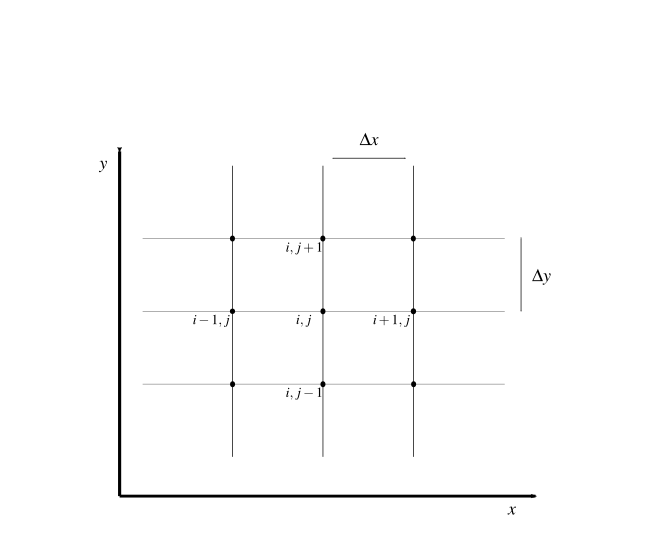
\includegraphics[width=95mm]{./Imagenes/malla-DF1}
		\caption[Discretización por Diferencias Finitas]{Discretización espacial (malla) por el método de diferencias finitas \cite{anderson-yotros}}
		\label{malla-DF1}
	\end{figure}
	
	\paragraph*{}
	Todos los términos de la serie truncados se agrupan en un sólo término conocido como error de truncamiento y es representado por la simbología $O()$. Volviendo a la ecuación (\ref{taylor-forward}) y resolviendo para $\left( \pdv{f}{x} \right)_{i,j}$ tenemos:
	
	\begin{equation}
	\left( \pdv{f}{x} \right)_{i,j} = \frac{f_{i+1, j} - f_{i,j}}{\Delta x} - \left( \pdv[2]{f}{x} \right)_{i,j} \frac{\Delta x}{2} - \left( \pdv[3]{f}{x} \right)_{i,j} \frac{(\Delta x)^2}{6} - \dotsb
	\end{equation}
	o bien:
	\begin{equation*}
	\left( \pdv{f}{x} \right)_{i,j} = \frac{f_{i+1, j} - f_{i,j}}{\Delta x} + O(\Delta x)^2
	\end{equation*}
	que para simplificar, queda:\\
	\begin{equation}
	\left( \pdv{f}{x} \right)_{i,j} = \frac{f_{i+1, j} - f_{i,j}}{\Delta x}
	\label{forward-x1}
	\end{equation}
	
	\paragraph*{}
	El símbolo $O(\Delta x)$ representa el error de truncamiento de la serie de expansión, y para este caso particular se dice que tiene una precisión de primer orden, ya que se están despreciando los términos de orden superior.
	
	\paragraph*{}
	La ecuación \ref{forward-x1} se le conoce como una aproximación tipo ``forward'' de primer orden y representa el valor aproximado del valor de la derivada parcial $\left( \pdv{f}{x}\right)_{i,j}$ calculada mediante la relación lineal del punto $(i,j)$ con el punto $(i+1,j)$. (Figura \ref{fig:grafica-forward})
	
	\begin{figure}[htbp!]
		\centering
		\subfigure[Aproximación forward]{\label{fig:grafica-forward}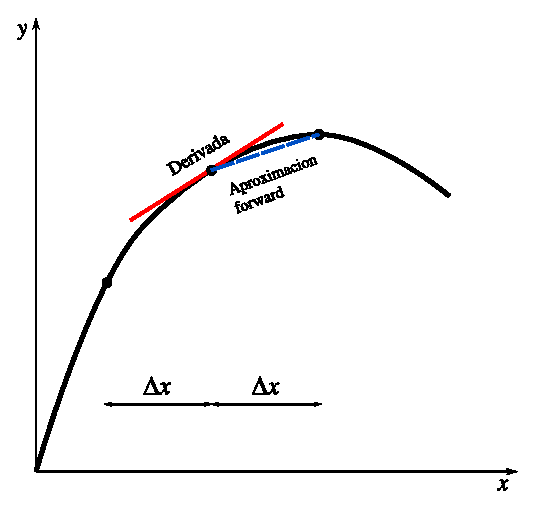
\includegraphics[width=65mm]{./Imagenes/grafica-forward}}
		\subfigure[Aproximación backward]{\label{fig:grafica-backward}\includegraphics[width=65mm]{./Imagenes/grafica-backward}}
		\subfigure[Aproximación central]{\label{fig:grafica-central} 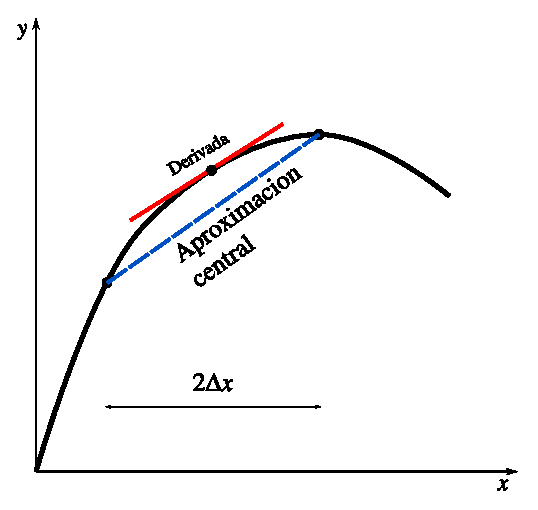
\includegraphics[width=65mm]{./Imagenes/grafica-central}}
		\caption[Aproximaciones por Diferencias Finitas]{Esquemas de las aproximaciones por el método de diferencias finitas.\cite{chapra}}
	\end{figure}
	
	\paragraph*{}
	Para obtener una aproximación tipo ``backward'' se debe generar una serie de Taylor para el punto $(i-1, j)$ expandiendo a partir del punto $(i, j)$
	\begin{equation}
	f_{i-1, j} = f_{i,j} + \left( \pdv{f}{x}\right)_{i,j} \Delta x + \left( \pdv[2]{f}{x} \right)_{i,j} \frac{(-\Delta x)^2 }{2\,!}  + \left( \pdv[3]{f}{x} \right)_{i,j} \frac{(-\Delta x)^3}{3\,!} + \dotsb + \left( \pdv[n]{f}{x} \right)_{i,j} \frac{(-\Delta x)^n}{n\,!}
	\label{taylor-backward}
	\end{equation}
	\paragraph{}
	Una vez generada la serie, se sigue el mismo procedimiento empleado en la derivación de la aproximación ``forward'' para obtener:
	\begin{equation}
	\left( \pdv{f}{x} \right)_{i,j} = \frac{f_{i,j} - f_{i-1,j}}{\Delta x}
	\label{backward-x1}
	\end{equation}
	\\que es la ecuación de una aproximación ``backward''. (Figura \ref{fig:grafica-backward})
	
	\paragraph*{}
	Para diferentes aplicaciones de DFC, no basta con tener aproximaciones con precisión de primer orden, por lo cual se opta por generar una ecuación que tenga una precisión de segundo orden, a esta se le conoce como ``aproximación central de segundo orden''. La deducción de ésta, parte de la resta de la ecuación \ref{taylor-forward} y la ecuación \ref{taylor-backward}, que da como resultado:
	\begin{equation}
	f_{i+1,j} - f_{i-1, j} = 2 \left( \pdv{f}{x} \right)_{i,j} \Delta x + 2 \left( \pdv[3]{f}{x} \right)_{i,j} \frac{(\Delta x)^3}{3 \,!} + \dotsb + 2 \left( \pdv[n]{f}{x} \right)_{i,j} \frac{(\Delta x)^n}{n\,!}
	\end{equation}
	que se puede simplificar a:\\
	\begin{equation}
	\left( \pdv{f}{x} \right)_{i,j} = \frac{f_{i+1,j} - f_{i-1,j}}{2 \Delta x}
	\label{central-x1}
	\end{equation}
	se observa en la ecuación \ref{central-x1} que para obtener un coeficiente en el punto $(i,j)$ se está utilizando información proveniente de los nodos $(i-1, j)$ e $(i+1, j)$, adyacentes a dicho punto. (Figura \ref{fig:grafica-central})
	
	\paragraph*{}
	Para el análisis de flujos viscosos, además de los coeficientes que sustituyen a las derivadas parciales de primer orden se necesitan desarrollar aproximaciones para las derivadas parciales de segundo orden, dado que, en las ecuaciones que describen el flujo de fluidos viscosos, las ecuaciones de Navier-Stokes, los términos de mayor orden son derivadas parciales de segundo orden.
	
	\paragraph*{}
	Si se suman las ecuaciones \ref{taylor-forward} y \ref{taylor-backward}, se obtiene un coeficiente para $\pdv[2]{f}{x}$, como se muestra a continuación:
	\begin{equation*}
	f_{i+1,j} + f_{i-1, j} = 2 f_{i,j} + \left( \pdv[2]{f}{x} \right)_{i,j} \frac{(\Delta x) ^2}{2\,!} + \left( \pdv[4]{f}{x} \right)_{i,j} \frac{(\Delta x)^4}{4\,!} + \dotsb + \left( \pdv[n]{f}{x} \right)_{i,j} \frac{(\Delta x)^n}{n\,!}
	\end{equation*}
	despejando la segunda derivada parcial y despreciando el error de truncamiento:
	\begin{equation}
	\left( \pdv[2]{f}{x} \right) = \frac{f_{i+1,j} - 2f_{i,j} + f_{i-1,j}}{(\Delta x)^2}
	\label{central-x2}
	\end{equation}
	a la ecuación \ref{central-x2} se le conoce como aproximación central para la derivada de segundo orden.
	
	\paragraph*{}
	Ahora se desea obtener una aproximación por diferencias finitas para una derivada parcial mixta, llámese $\pdv{f}{x}{y}$, donde $f$ es una función dependiente de la posición de la partícula de fluido a lo largo de dos ejes, $x$ y $y$. Dado que:
	\begin{equation}
	\left( \pdv{f}{x}{y} \right) = \pdv{y} \left( \pdv{f}{x} \right)
	\end{equation}
	podemos desarrollar una aproximacion por diferencias ``central'' de la derivada parcial de $y$ en función de $x$, es decir:
	\begin{equation}
	\left( \pdv{f}{x}{y} \right)_{i,j} = \frac{\left( \pdv{f}{y} \right)_{i+1, j} - \left( \pdv{f}{y} \right)_{i-1,j}}{2 \Delta x}
	\end{equation}
	y desarrollando una diferencia central para la derivada parcial de $f$ con respecto a $y$ tenemos:
	\begin{equation}
	\left( \pdv{f}{x}{y} \right)_{i,j} = \frac{1}{2 \Delta x} \left[ \frac{f_{i+1, j+1} - f_{i+1, j-1}}{2 \Delta y} - \frac{f_{i-1, j+1} - f_{i-1, j-1}}{2 \Delta y} \right]
	\end{equation}
	\begin{equation}
	\left( \pdv{f}{x}{y} \right)_{i,j} = \frac{1}{4 \Delta x \Delta y} \left( f_{i+1, j+1} + f_{i-1, j-1} - f_{i+1, j-1} - f_{i-1, j+1} \right)
	\end{equation}
	
	\paragraph*{}
	La misma metodología se aplica para obtener las aproximacinoes por el método de diferencia finitas de una función respecto a un eje cualquiera, llámese eje $y$, $\xi$ o $\eta$.
	
	\paragraph*{}
	La mayor ventaja que presenta el método de diferencias finitas es su simplicidad de implementación, aunque presenta una limitante, el método únicamente es aplicable a mallas estructuradas, además de tampoco poderse aplicar a cuerpos de geometría curvilíneas, por lo que es necesario hcer una transformación de la malla, de un dominio físico a un dominio lógico, como se analiza en el capítulo \ref{chap:mallas}.
	
	\paragraph*{}
	Es este último punto, la piedra angular en la importancia del desarrollo de métodos de generación de mallas, ya que se busca trabajar con mallas en las cuales, en sus sistema de coordenadas computacional, pueda ser aplciado el método de diferencias finitas para la solución de problemas.
	%
	%
	%
	%
	%
	
					
	% 
	%
	% 
	%
	%
	\chapter{Mallas}
	\label{chap:mallas}
	\paragraph*{}
		Las mallas proveen soporte matemático para llevar a cabo una solución numérica de las ecuaciones que gobiernan el campo de análisis como medio continuo. La solución numérica se obtiene superponiendo la malla sobre el medio continuo, discretizando las ecuaciones respecto a la malla y por último, aplicando un algoritmo numérico de solución a la discretización de las ecuaciones. Este proceso resulta ser una evaluación de la solución en los nodos de la malla.
	\paragraph*{}
		La mecánica de fluidos trabaja con ecuaciones no lineales, las cuales describen los flujos de fluidos, dichas ecuaciones en la mayoría de los casos prácticos de análisis no pueden ser resueltas de una manera analítica, por lo que se ha optado por la solución de dichas ecuaciones mediante métodos de aproximaciones entre los cuales encontramos los métodos de expansión y perturbación, método de diferencias finitas, método de volúmenes finitos e incluso el método de elementos finitos. En general los de mayor aplicación práctica son los tres últimos, pero para poder usarlos es necesario discretizar el campo de análisis mediante el uso de una malla.\cite{thompsonhandbook}
	\paragraph*{}
		La utilización del método de diferencias finitas es directa si el problema se puede expresar en un sistema de coordenadas cartesianas, aunque el mismo puede aplicarse a sistemas de coordenadas polares, cilindricas o esféricas, dando como resultado una malla rectangular estructurada, con espaciamiento uniforme entre los nodos en la dirección de los ejes del sistema. La mayoría de casos prácticos de interés en la DFC, tratan con geometrías complejas, lo que hace que sea muy dificil, si no imposible, generar una malla en alguno de los sitemas de cordenadas antes mencionados, que ajuste en su frontera interna de manera exacta a la forma de la geometría a analizar. Esto presenta una limitante que se debe atender, se debe llevar a cabo una transofrmación de sistemas de coordenadas, llevando el dominio físico del problema a un dominio computacional. (Figura \ref{fig:dominios}) El dominio computacional es una abstración matemática, mientras que el dominio físico es el dominio continuo para el cual se desea una solución numérica. 
	\begin{figure}[htbp!]
		\centering
		\includegraphics[width=170mm]{./Imagenes/dominios}
		\caption[Dominios lógico y físico]{Dominios lógico (izquierda) y físico (derecha). \cite{numerical-grid}}
		\label{fig:dominios}
	\end{figure}
	\paragraph*{}
		Una malla es un conjunto de puntos destribuidos a lo largo de un campo dentro del cuál se llevaran a cabo los cálculos para obtener la solución de ecuaciones diferenciales parciales. Existen dos tipos principales de mallas: estructuradas y no estructuradas. (Figura \ref{fig:malla-estructurada-noestructurada}) Las mallas estructuradas se forman mediante la intersección de coordenadas curvilíneas, formando celdas cuadriláteras en dos dimensiones, o hexahedros en tres dimensiones. En contraste, las mallas no estructuradas no tienen relación alguna con las direcciones coordenadas del sistema, éstas consisten generalmente de triángulos y tetahédros en dos y tres dimendiones respectivamente, aunque en realidad se puede hacer uso de calquier forma geométrica. Para este trabajo se considerará el desarrollo  de  mallas estructuradas principalente, que en principio tendrán una forma curvilinea ajustada a la forma del perfil alar con el que se esté trabajando como frontera interna del dominio.
	\begin{figure}[htbp!]
		\centering
		\subfigure[Malla Estructurada]{\label{fig:malla-estructurada}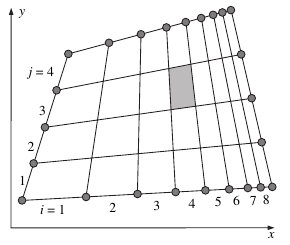
\includegraphics[width=50mm]{./Imagenes/malla-estructurada}} \hspace{20mm} %marca separación entre subfiguras
		\subfigure[Malla no Estructurada]{\label{fig:malla-no-estructurada}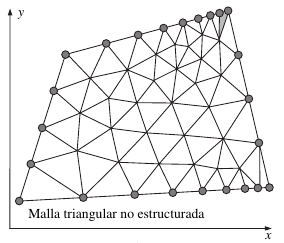
\includegraphics[width=50mm]{./Imagenes/malla-no-estructurada}}
		\caption[Mallas estructuradas y no estructuradas]{Mallas estructuradas y no estructuradas. \cite{cengel}}
		\label{fig:malla-estructurada-noestructurada}
	\end{figure}
	
	
	\paragraph*{}
		La malla debe de generarse bajos ciertas restricciones las cuales suelen ser difíciles de satisfacer por completo. En la actualidad el tiempo que toma generar una malla llega a ser mayor en órdenes de magnitud que el tiempo requerido para la construcción y análisis de la solución del flujo sobre la malla. En especial ahora que hay mayor disponibilidad de software para la solución de flujos.\cite{thompsonhandbook}
	
	
	\section{Tipos de Mallas}
		\paragraph*{}
		Existen tres tipos base de mallas conocidos como mallas C, H u O respectivamente. El nombre que dichos tipos de mallado reciben se debe a que su estructura asemeja a dichas letras (en mayúsculas) desde una vista de planta.
		
		\begin{figure}[htbp!]
			\centering
			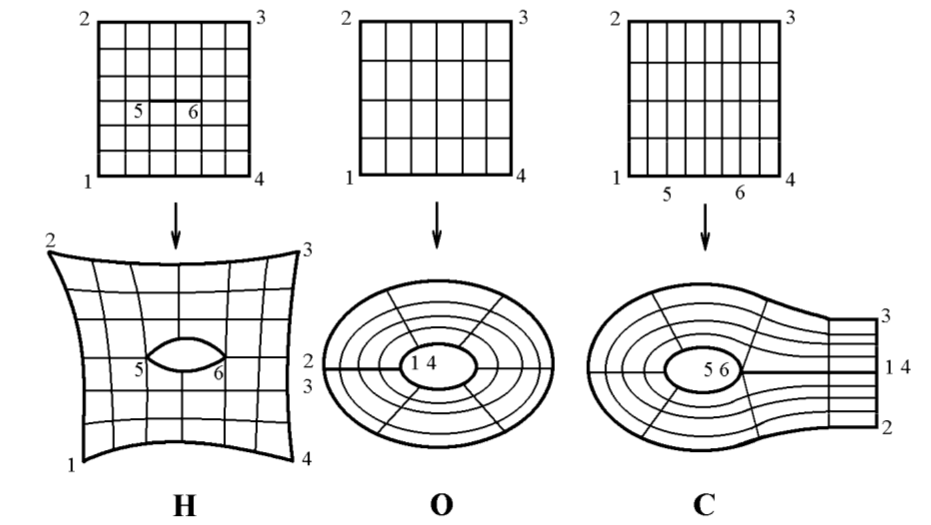
\includegraphics[width=170mm]{./Imagenes/tipos-de-malla}
			\captionsetup{justification=centering, margin=2cm}
			\caption[Tipología de mallas]{Tipología de malla y sus respectivos espacios computacionales. H(izquierda), O(centro), C(derecha).\cite{vladimir-grid}}
			\label{fig:tipos-de-malla}
		\end{figure}
		
		\subsection{Mallas tipo C}
			\paragraph*{}
				Las mallas tipos C están compuestas por una sección semicircular y otra rectangular en la frontera exterior, mientras que la frontera interior es de la misma forma del objeto que se analiza.
			\paragraph*{}
				Suelen utilizarse para el análisis de flujos alrededor de perfiles alares, pues ofrecen como principal ventaja un buen análisis del flujo en la zona de deflexión de la estela, en especial si se compara contra las mallas tipo O.\cite{best-practices-grid-generation}
			\paragraph{}
				La transformación de esta malla de un espacio físico a un espacio computacional da como resultado una malla conformada por rectangulos. Durante la transformación se debe identificar un segmento, tambien conocido como corte, ya que este proceso implica conceptualemte, una separación en dicho corte, para posteriormente deformar el espacio físico llevándolo así a convertirse en una malla estructurada uniforme. En la figura \ref{fig:malla-c} se observa que en el dominio físico, el segmento $(ab)$ representa la sección del mallado donde se realiza el corte y que tambien se le llama $(a'b')$, y que en el dominio computacional este segmento representa dos segmentos diferentes.
				\begin{figure}[htbp!]
					\centering
					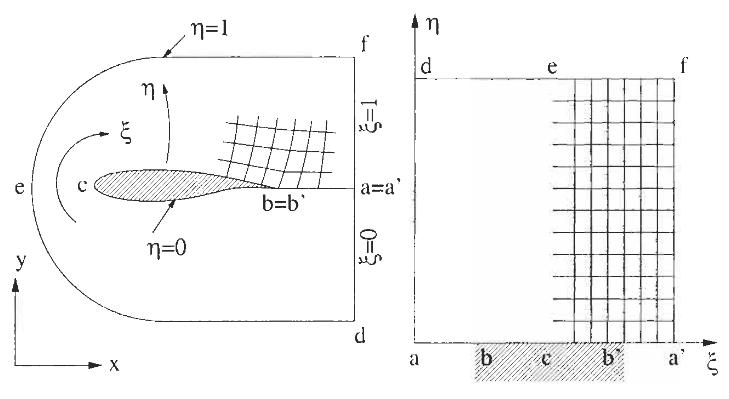
\includegraphics[width=155mm]{./Imagenes/malla-c}
					\captionsetup{justification=centering, margin=2cm}
					\caption[Malla tipo C]{Malla tipo C y su transformación del espacio físico (izquierda) al espacio lógico (derecha). \cite{blazek}}
					\label{fig:malla-c}
				\end{figure}
		\subsection{Mallas tipo O}
			\paragraph*{}
				Este tipo de mallas son principalmente de sección circular, de ahí su nombre. Suelen ser utilizadas para el análisis del flujo alrededor de algunos componentes de aeronaves, como puede ser el fuselaje o las góndolas, entre otros.\cite{vladimir-grid} Tambien pueden llegar a utilizarse en el análisis de perfiles alares, pero presentan la dificultad de ofrecer una baja calidad de mallado en el borde de salida.\cite{blazek}\cite{best-practices-grid-generation}
			\paragraph*{}
				En este caso, al igual que sucede con las mallas tipo C, el resultado en el dominio lógico es un cuadrado.El proceso de transformación de este tipo de malla se puede conceptualizar como el desdoble del espacio físico a partir de un corte, en la figura \ref{fig:malla-o} se representa como $(ac)$ o como $(a'c')$, para después deformarlo hasta alcanzar la forma cuadrada esperada.
			\begin{figure}[htbp!]
				\centering
				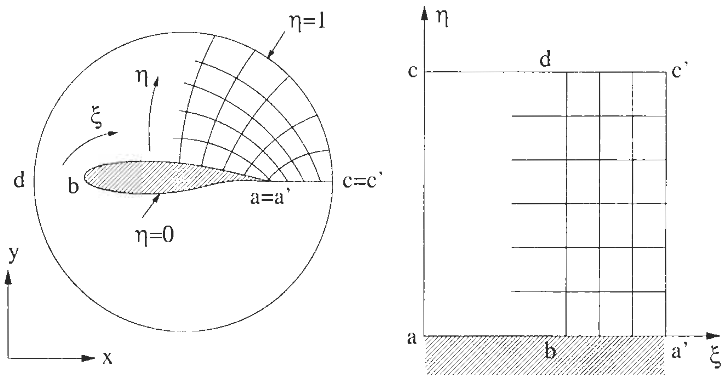
\includegraphics[width=170mm]{./Imagenes/malla-o}
				\captionsetup{justification=centering, margin=2cm}
				\caption[Malla tipo O]{Malla tipo O y su transformación del espacio físico (izquierda) al espacio lógico (derecha). \cite{blazek}}
				\label{fig:malla-o}
			\end{figure}
		\subsection{Mallas tipo H}
			\paragraph*{}
				Este tipo de mallas son utilizadas principalmente en los análisis de tubomaquinaria, específicamente en la zona de los alabes.\cite{blazek}\cite{best-practices-grid-generation} Tambien suelen utilizarse en el análisis de alas de aeronaves. \cite{vladimir-grid}
			\paragraph*{}
				La transformación en este tipo de malla, tambien da como resultado un dominio computacional cuadrado, que puede tener o no un corte al interior el cual corresponde a la frontera interior del dominio físico. (Figura \ref*{fig:tipos-de-malla}(H)) La frontera externa del dominio computacional corresponde a la frontera externa del dominio físico.
			
			\paragraph*{} 
			La figura \ref{fig:malla-h} muestra el uso de una malla tipo H para el análisis del flujo a través de los álabes de una turbina, y su transformación del dominio físico al computacional. En este caso no existe un cuerpo en el centro del mallado, por lo que no hay corte alguno en el dominio lógico.
			\begin{figure}[htbp!]
				\centering
				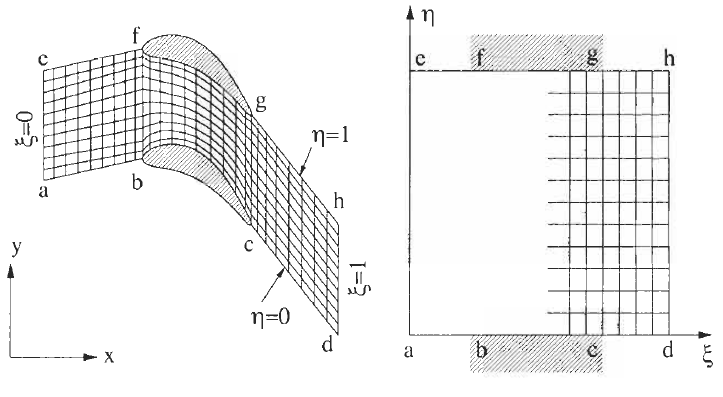
\includegraphics[width=170mm]{./Imagenes/malla-h}
				\captionsetup{justification=centering, margin=2cm}
				\caption[Malla tipo O]{Malla tipo H y su transformación del espacio físico (izquierda) al espacio lógico (derecha). \cite{blazek}}
				\label{fig:malla-h}
			\end{figure}
			
			\paragraph*{}
			En el caso de que se quiera ocupar una malla H con un cuerpo a analizar en el interior del dominio, como el caso representado en la figura \ref*{fig:tipos-de-malla}(H) se puede realizar un mallado uniforme, quizás mediante un método de interpolación algeráica, sobre el dominio físico quedando así coincidente con el dominio computacional. Los puntos 5 y 6 requieren de un trato especial al momento de llevar a cabo la solución, un ejemplo de esto puede ser que todos los puntos del mallado que caen dentro del objeto de análisis no sean utilizados durante la solución.
			
	\section{Consideraciones preliminares para la generación de mallas}	
		\paragraph*{}
			La densidad de la malla es el primer aspecto que se debe considerar, se debe generar una malla solo sufcientemente densa para que la aproximación numérica sea precisa, sin embargo, se debe tener cuidado en no hacer la malla demasiado densa, tanto que resulte impractico llevar a cabo un análisis y llegar a una eventual solución.
		\paragraph{}
			 Otro importante aspecto a tener en cuenta durante este proceso, es la eficiencia computacional. Por un lado el uso de memoria podría ser tan grande que resulte impractico llevar a cabo este proceso, por lo que una organización adecuada de la información es de vital importancia. Por otro lado, la generación de mallas debe llevarse a cabo mediante la implementación de códigos lo menos complejos posible.
			
	\section{Técnicas de generación del mallado}
		\paragraph*{}
			La generación de mallas \textit{per se}, es un proceso libre durante su desarrollo, es decir, no se lleva a cabo mediante alguna fórmula o procedimiento estricto, por lo tanto, cualquier desarrollo se puede considerar apto para este propósito siempre y cuando dé como resultado una mallado adecuado para el análisis que se pretende realizar. Sin embargo, si hay ciertas consideraciones a tomar en cuenta, tales como la capacidad de manejar problemas con múltiples variables, las cuales podrían variar en varios órdenes de magnitud. Del mismo modo, se debe considerar la posibilidad de presentar factores de compresión en ciertas áreas de la malla, en contraste con una malla uniforme.
			
		\paragraph*{}
			Podemos señalar principalmente dos tipos de técnicas para la generación de mallado, de entre el amplio número de técnicas existentes al día de hoy, las cuales son:
			\begin{itemize}
				\item Métodos algebráicos: es de todos, el método más sencillo de implementar, una de sus ventajas es la rapidez con la que se genera la malla. Se utiliza un método de interpolación para determinar los nodos del mallado, partiendo de las coordenadas de la frontera externa e interna. Y se realiza la transformación del dominio físico al lógico mediante una ecuación algebráica.
				\item Metódos mediante  ecuaciones diferenciales parciales (EDP): se resuelve una EDP para obtener la distribución de los nodos, la resolución de las mismas se lleva a cabo mediante aproximaciones por el método de diferencias finitas.  La distribución de la malla puede ser uniforme o concentrada dependiendo del tipo de ecuación que se resuelva.
			\end{itemize}
%
%
%
%
%		

%
%
%
%
%
\chapter{Generación de mallas mediante métodos algebráicos}
	\paragraph*{}
		Como ya se mencionó previamente, los métodos más eficientes para la generación de mallas son los métodos algebráicos. Éstos métodos basados en interpolación son de gran utilidad en la industria, debido a su sencilla implementación, además de la capacidad de control sobre la densidad de la malla respecto a un nodo dentro del dominio. Un aspecto en contra de la generación de mallas mediante estos métodos es que no tienen la capacidad de suavizar las curvas, si no que tienden a mantener la forma de las fronteras, por lo que si se llegara a presentar algún tipo de discontinuidad en la frontera interna (superficie de análisis), esta seguiría presente los nodos internos de la malla. Es por esto que estos métodos son utilizados de manera general, como una primera aproximación, la cual sirve como condición inicial en la generación de mallas mediante la solución de sistemas de ecuaciones diferenciales parciales.\cite{farrashkhalvat}
	\paragraph*{}
		La idea fundamental sobre la cual se desarrollan todos los métodos algebráicos es el uso de funciones de interpolación matemática para interpolar entre algunos puntos conocidos o previamente asignados (fronteras) para así obtener la distribución de puntos que se ubican entre los ya mencionados. El método de interpolación puede variar dependiendo del método algebráico que se esté empleando, pero la idea base permanece. \cite{siladic-grid-generation}
	\paragraph*{}
		Los métodos algebráicos relacionan un dominio computacional, descrito por un cuadrado en 2D y un cubo en 3D, con un dominio físico de geometría arbitraria.
		
		
	\section{Interpolación unidireccional}
		\paragraph*{}
			La interpolación unidireccional se lleva a cabo interpolando una línea a la vez, en una dirección del espacio computacional, ya sea $\xi$ o $\eta$. Es decir, para interpolar en la dirrección $\xi$ (desarrollo que se presenta en este trabajo), se deben seleccionar puntos en las frontera tanto interna como externa, que correspondan a la misma línea $\eta = constante$ y a lo largo de la cual se hará la interpolación, haciendo la variación en la coordenada $\xi$, interpolando así, línea por línea hasta terminarse de generar la malla. El mismo procedimiento se puede llevar a cabo interpolando en la dirección de $\eta$.
		\subsection{Interpolación Polinomial}\label{Lagrange}
			\paragraph*{}
				En este método se ocupa el polinomio de Lagrange como ecuación de interpolación para generar la malla.
				\begin{align}
					L_{i}(x) = \frac{ (x - x_{0} )(x - x_{1}) \dotsb (x - x_{i-1}) (x - x_{i+1}) \dotsb (x - x_{n}) }{(x_{i} - x_{0} )(x_{i} - x_{1}) \dotsb (x_{i} - x_{i-1}) (x_{i} - x_{i+1}) \dotsb (x_{i} - x_{n}) } && i = 0, 1, \dotsc , n
				\end{align}
				\\El polinomio resultante será de grado $n$, donde el numerador omite el término $(x - x_{i})$
			
			\paragraph*{}
				El caso más sencillo con el que se puede trabajar el polinomio de Lagrange es generando un polinomio de grado 1, que resulta ser una línea recta que pasa a través de dos puntos $(x_{0} , y_{0})$ y $(x_{1}, y_{1})$, los cuales pertenecen a la frontera interna y externa respectivamente. Para este caso, se tienen los siguientes términos:
				\begin{align*}
					L_{0} = \frac{ ( x - x_{1} ) }{ (x_{0} - x_{1} ) } && L_{1} = \frac{ ( x - x_{0} ) }{ (x_{1} - x_{0} ) }
				\end{align*}
				dando como resultado la ecuación que describe a una recta
				\begin{equation}
					y = y_{0} \frac{ ( x - x_{1} ) }{ ( x_{0} - x_{1} ) }  + y_{1} \frac{ (x - x_{0})  }{( x_{1} - x_{0} )} = y_{0} (1 - \xi) + y_{1}\xi
				\end{equation}
				de donde se sabe que
				\begin{equation}
					\xi = \frac{x - x_{0}}{x_{1} - x_{0}}
					\label{xi}
				\end{equation}
				y se observa que $\xi = 0, 1$ cuando $x = x_{0}, x_{1}$ respectivamente.
			\paragraph*{}
				Despejando $x$ de la ecuación \ref{xi} se obtiene:
				\begin{equation}
					x = (x_{1} - x_{0})\xi - x_{0} = x_{0}(1 - \xi) + x_{1}\xi
				\end{equation}
				por lo que la ecuación constitutiva de éste método, para una interpolación en dirección del eje $\xi$ del espacio computacional puede escribirse de la siguiente manera:
				\begin{equation}
					r(\xi, \eta_{j}) = (1 - \xi_{i}) r(0, \eta_{j}) + \xi_{i}r(1, \eta_{j})
				\end{equation}
				
			\paragraph*{}
				Se puede hacer uso de la generación de un polinomio de mayor grado, para lo cual se deben proporcionar más puntos previamente definidos por los cuales tiene que pasar la curva descrita del polinomio. Para generar una ecuación de grado $n$ se deben proporcionar como datos de inicio, al menos $n+1$, es decir, si se quisiera hacer la interpolación mediante un polinomio de grado 2, se debe proporcionar la información de al menos 3 puntos. Siempre cabe la posibilidad de que los puntos pertenezcan a una linea recta, en cuyo caso los términos de mayor orden se verán eliminados.
			\paragraph*{}
				Las figuras \ref{fig:malla-inter} y \ref{fig:malla-inter-cerca} presentan una malla y su vista de detalle generada mediante este método alrededor de un perfil aerodinámico.				
				\begin{figure}[htbp!]
					\centering
					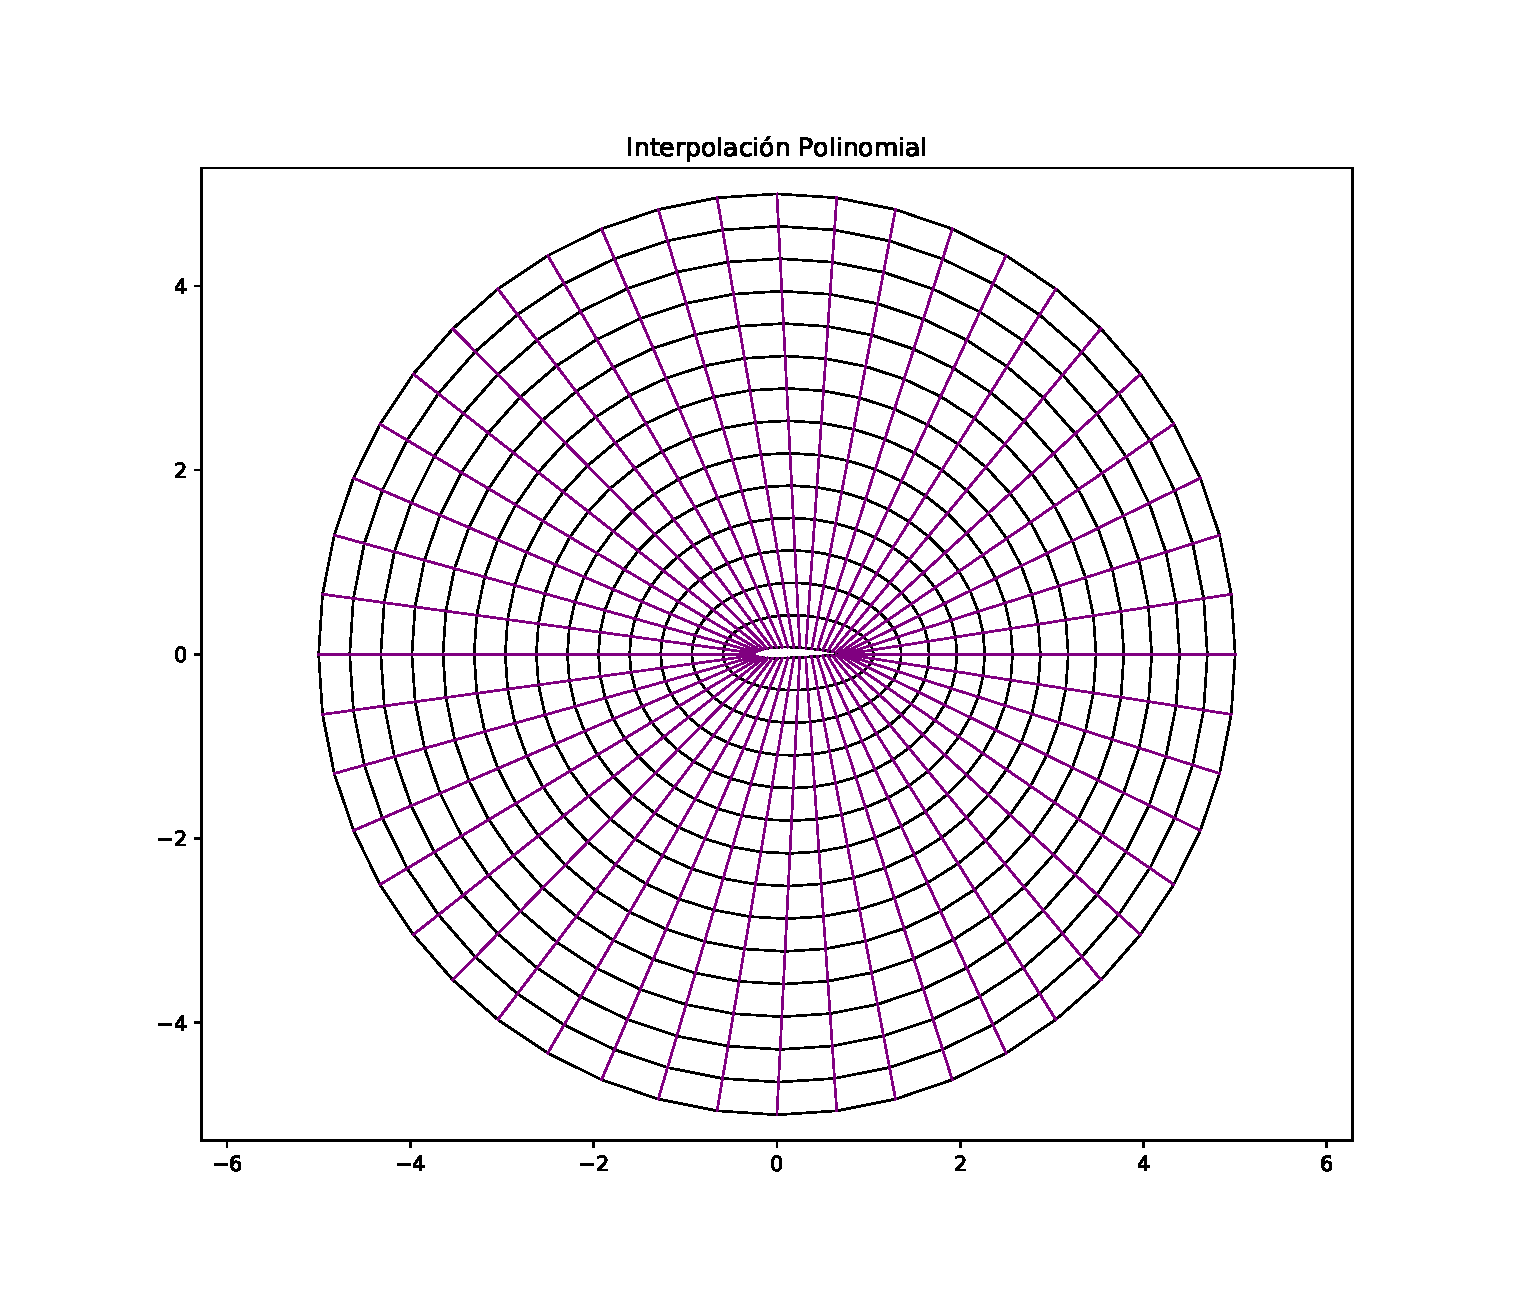
\includegraphics[width=120mm]{./Imagenes/M-inter_pol}
					\captionsetup{justification=centering, margin=2cm}
					\caption[Malla Interpolación Polinomial]{Malla tipo O generada mediante el método de interpolación polinomial alrededor de un perfil NACA 2412. Densidad de malla $49$X$15$}
					\label{fig:malla-inter}
				\end{figure}
				\begin{figure}[htbp!]
					\centering
					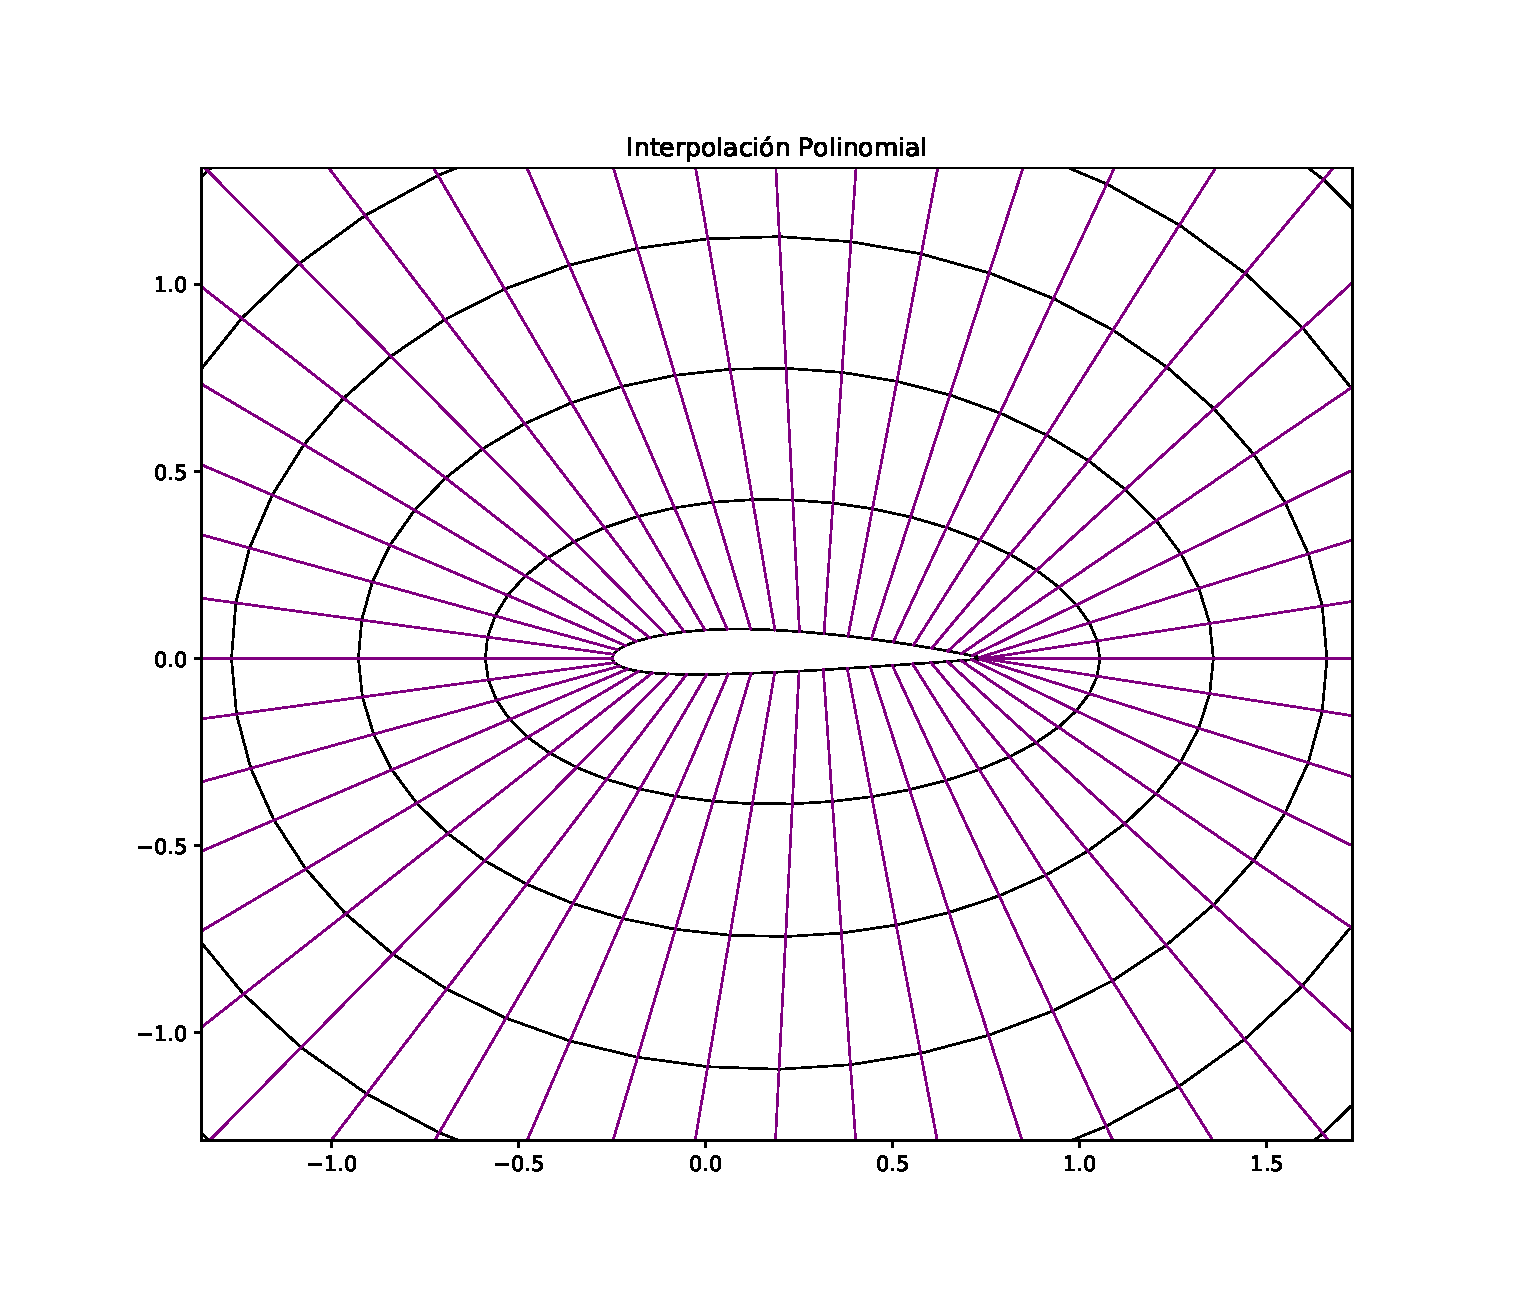
\includegraphics[width=120mm]{./Imagenes/M-inter_pol_cerca}
					\captionsetup{justification=centering, margin=2cm}
					\caption[Malla Interpolación Polinomial Acercamiento]{Vista de acercamiento a la malla generada de la figura \ref{fig:malla-inter} }
					\label{fig:malla-inter-cerca}
				\end{figure}
		
		\subsection{Interpolación mediante polinomios de Hermite}
			\paragraph*{}
				La interpolación mediante el polinomio de Lagrange se realiza mediante el uso de valores conocidos de ciertos puntos, sin embargo, es posible generar una malla partiendo tanto de valores conocidos de una función como de los valores de su primer derivada para ciertos puntos dados. El polinomio que describe este método se escribe como:
				\begin{equation}
					p(x) = \sum_{i = 0}^{n} y_{i}H_{i}(x) + \sum_{i = 0}^{n}y_{i}\prime \widetilde{H}_{i}(x)
				\end{equation}
			
			\paragraph*{}
				Los siguientes polinomios definen los polinomios de Hermite $H_{i}(x), \widetilde{H}_{i}(x)$ en función de polinomios de Lagrange:
				\begin{equation}
					H_{i}(x) = \{  1 - 2L\prime_{i}(x_{i})(x - x_{i})  \} \left[L_{i}\right]^2
				\end{equation}
				\begin{equation}
					\widetilde{H}_{i}(x) = (x - x_{i}) \left[L_{i}\right] ^ 2
				\end{equation}
			\paragraph*{}
				Se suele usar polinomios de Hermite cubicos, para los cuales se requiere el uso de polinomios de Lagrange de primer grado, es decir polinomios lineales. La ecuación constitutiva de la interpolación en dirección del eje $\xi$, por polinomios cúbicos de Hermite queda expresada de la siguiente manera:
				\begin{equation}
					r(\xi) = \sum_{i = 0}^{n} r_{i}H_{i}(\xi) + \sum_{i = 0}^{n} r\prime_{i}\widetilde{H}_{i}(\xi)
				\end{equation}
				que a su vez, desarrollando las operaciones matemáticas, se expresa como:
				\begin{align}
					&\begin{aligned}
						r(\xi, \eta_{j}) =& r(0, \eta_{j})(2\xi^3 - 3\xi^2 +1) + r(1, \eta_{j})(3\xi^2 - 2\xi^3) \\ &+ r\prime(0, \eta_{j})(\xi^3 - 2\xi^2 + \xi) + r\prime(1, \eta_{j})(\xi^3 - \xi^2)
					\end{aligned}
				\end{align}
				
	\section{Interpolación multidireccional}
		\paragraph*{}
			La interpolación multidireccional consiste en la obtención de una ecuación algebráica que permita la interpolación simultánea en 2 o más direcciones. Para este caso (2D), se generan ecuaciones que permitan la interpolación simultánea, en el espacio computaciones, en ambas direcciones $\xi$ y $\eta$.
		\subsection{Interpolación Transfinita - TFI}
			\paragraph*{}
				El método de TFI es un método de interpolación multivariable. Cuando se aplica el TFI para la generación de mallas, se restringe la malla para que coincida con la fronteras especificadas. Este método consiste en la suma de las interpolaciones de una sola variable para cada una de las coordenadas computacionales. Existen diversos tipos de interpolación a lo largo de una coordena, por lo que existen práctimanete un número ilimitado de variantes de TFI creadas a partir de la combinación de diversas interpolaciones de una sola variable.\cite{thompsonhandbook}
			\paragraph*{}
				Una de las principales ventajas del método de interpolación transfinita es que asegura una concordancia en las fronters en ambas direcciones. Su escencia es la de la interpolación en cada una de las coordenadas computacionales, formando así los productos tensores de las interpolaciones, y finalmente, se lleva a cabo una suma ``booleana''. Las interpolaciones unidireccionales son una combinación lineal de datos proporcionados por el usuarios del dominio físico para valores dados de las coordenadas del dominio lógico.
			\paragraph*{}
				A partir de la existencia de una transformación $r = r(\xi, \eta)$ ($x = x(\xi, \eta), y = y(\xi, \eta)$ la cual hace un mapeo de un cuadrado de dimensiones $0 < \xi < 1, 0 < \eta < 1$ en el dominio computacional, con la región del dominio físico, delimitada por una frontera externa y una interna, que se pretende analizar. De igual modo, se puede escribir otra transformación $P_{\xi}$, la cual recibe el nombre de proyector, la cual relaciona puntos en el espacio lógico con puntos en el espacio físico, definida como:
				\begin{equation}
					P_{\xi}(\xi, \eta) = (1 - \xi)r(0, \eta) + \xi r(1, \eta)
				\end{equation}
			\paragraph*{}
				Como ya se explicó en la sección \ref{Lagrange}, esta tranformación hace una transformación con la cual las fronteras en la dirección de $\xi$ son mapeadas, mientras que las fronteras en dirección de $\eta$ son reemplazadas por lineas rectas. De manera análoga se puede definir el proyector:
				\begin{equation}
					P_{\eta}(\xi, \eta) = (1 - \eta)r(\xi, 0) + \eta r(\xi, 1)
				\end{equation}
				con el cual se preservan las fronteras en dirección $\eta$ y se reemplazan las fronteras en $\xi$ por líneas rectas.
			\begin{figure}[htbp!]
				\centering
				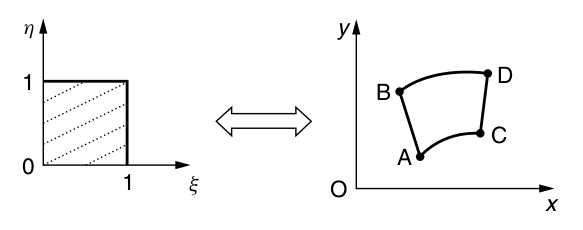
\includegraphics[width=120mm]{./Imagenes/mapeo_eta}
				\caption[Transformación de malla por $P_{\eta}$]{Transormación de una malla a través del proyector $P_{\eta}$ \cite{farrashkhalvat}}
				\label{fig:mapeo_eta}
			\end{figure}
			\paragraph*{}
				La figura \ref{fig:mapeo_eta} representa gráficamente la transformación de la malla del dominio lógico al dominio computacional mediante la aplicación del proyector $P_{\eta}$. Se observa como las fronteras conformadas por los segmentos $AC$ y $BD$ se conservan durante las transformación, mientras que las fronteras $AB$ y $CD$ son reemplazadas por líneas rectas.
			\paragraph*{}
				A partir de estas ecuaciones, se uede definir un mapeo compuesto $P_{\xi}P_{\eta}$, de tal manera que:
				\begin{align}
					\begin{aligned}
						P_{\xi}(P_{\eta}(\xi, \eta)) &= P_{\xi} ((1 - \eta)r(\xi, 0) + \eta r(\xi, 1)) \\
						&= (1 - \xi) \left[ (1 - \eta)r(0, 0) + \eta r(0, 1) \right] + \xi \left[ (1 - \eta)r(1, 0) + \eta r(1,1) \right]\\
						&= (1 - \xi)(1 - \eta)r(0, 0) + (1-\xi)\eta r(0, 1) + \xi(1 - \eta)r(1, 0) + \xi\eta r(1, 1)
					\end{aligned}
				\end{align}
			\paragraph*{}
				Con esta transformación compuesta, se logra preservar los 4 vértices en los que se interseccionan las fronteras, sin embargo, las cuatro fronteras son reemplazadas por líneas rectas. Es decir, las líneas $\xi = constante$ y $\eta = constante$ en el dominio computacional son transformadas como líneas rectas en el dominio físico, como se muestra en la figura \ref{fig:mapeo_xieta}.
			\begin{figure}[htbp!]
				\centering
				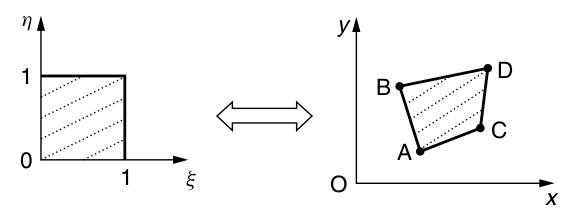
\includegraphics[width=120mm]{./Imagenes/mapeo_xieta}
				\caption[Transformación de malla por $P_{\xi}P_{\eta}$]{Transormación de una malla a través del proyector compuesto $P_{\xi}P_{\eta}$ \cite{farrashkhalvat}}
				\label{fig:mapeo_xieta}
			\end{figure}
			
			\paragraph*{}
				Si consideramos los diferentes mapeos de un lado, bajo cualquiera de los proyectores previamente desarrollados, por ejemplo el lado $\eta = 0$, bajo el proyector $P_{\xi}$ es mapeado con una línea recta $AC$, si por otro lado se lleva a cabo la transformación medainte el proyector $P_{\eta}$ el mapeo resultante es uno a uno, es decir que la recta $\eta = 0$ se mapea con la curva de la frontera $AC$. Por último, transformando con el proyector compuesto $P_{\xi}P_{\eta}$ tambien se hace un mapeo con la línea recta $AC$.
			\paragraph*{}
				Desarrollando la misma lógica y consideraciones a las 4 fronteras de la frontera, se concluye que el mapeo compuesto $(P_{\xi} + P_{\eta} - P_{\xi}P_{\eta})$ lleva a cabo una transformación con un mapeo uno  a uno de las fronteras del cuadrado de longitud uitaria (dominio computacional) con la curvas de frontera del dominio físico. A este mapeo se le conoce como la suma booleana de las transformaciones $P_{\xi}$ y $P_{\eta}$, y se escribe $P_{\xi}\oplus P_{\eta}$, por lo tanto:
				\begin{equation}
					P_{\xi}\oplus P_{\eta} = P_{\xi} + P_{\eta} - P_{\xi} P_{\eta}
				\end{equation}
				con lo que la fórmula final queda:
				\begin{align}
					\begin{aligned}
						\left( P_{\xi}\oplus P_{\eta} \right)(\xi, \eta) =& P_{\xi}(\xi, \eta) + P_{\eta}(\xi, \eta) - P_{\xi}P_{\eta}(\xi, \eta) \\
						=& (1 - \xi)r(0, \eta) + \xi r(1, \eta) + (1 - \eta)r(\xi, 0) + \eta r(\xi, 1) \\&- (1-\xi)(1 - \eta)r(0, 0) - (1 - \xi)\eta r(0, 1) - (1- \eta)\xi r(1, 0) \\& - \xi \eta r(1,1)
					\end{aligned}
				\end{align}
			\paragraph*{}
				Esta ecuación es la base del métro de TFI para dos dimensiones. La malla se genera tomando valores discretos $\xi_{i}, \eta_{j}$ para los ejes $\xi$ y $\eta$.
				


%
%
%
%
%

%
%
%
%
%
\chapter{Generación de mallas mediante EDP}
		\paragraph*{}
		La generación de mallas mediante estos métodos se ha esparcido gracias a a la versatilidad que poseen y la relativa facilidad con la que pueden ser aplicados. La idea sobre la cual se desarrolla el método, es la de obtener la solución númerica de una ecuación diferencial parcial, esta solución representa las coordenadas de la malla, la cual debe coincidir en su frontera interna, con la forma geométrica del cuerpo que se pretende analizar.\cite{siladic-grid-generation}
		
		\section{Generación de mallas mediante EDP elípticas}
			\paragraph*{}
				Para la solución de un sistema de EDP elípticas se necesita cumplir la condición de tener definidas las condiciones de frontera a lo largo de todos los puntos pertenecientes a la misma, es decir, que se tengan condiciones de frontera de Dirichlet.
				La solución se obtiene mediante diferentes métodos numéricos iterativos, entre los que destacan el método de Jacobi, el método de Gauss-Seidel y métodos de sobre relajación.
				
			\paragraph*{}
				La idea es que se calculen las coordenadas $(\xi, \eta)$ y que la solución del sistema de ecuaciones genere las correspondientes coordenadas $(x, y)$ del dominio físico, con un mapeo uno a uno, es decir, que exista una relación adecuada entre el dominio computacional y el lógico.
				
			\paragraph*{}
				Considerando la ecuación de Laplace:
				\begin{subequations}
					\begin{equation}
						\xi_{xx} + \xi_{yy} = 0
					\end{equation}
					\begin{equation}
						\eta_{xx} + \eta_{yy} = 0
					\end{equation}
					\label{ec-laplace}
				\end{subequations}\\
				donde como ya se ha mencionado, $\xi$ y $\eta$ representan las coordenadas del dominio computacional y además, son variables dependientes de $x$ y de $y$. Si se quiere trabajar con la forma inversa, es decir, que ahora $x$ y $y$ sean variables dependientes de $\xi$ y $\eta$, la ecuación  de Laplace se expresa como:
				\begin{subequations}
					\begin{equation}
						\alpha x_{\xi \xi} - 2\beta x_{\xi \eta} + \gamma x_{\eta \eta} = 0
					\end{equation}
					\begin{equation}
						\alpha y_{\xi \xi} - 2\beta y_{\xi \eta} + \gamma y_{\eta \eta} = 0
					\end{equation}
					\label{ec-laplace-invertida}
				\end{subequations}\\
				
				donde:
				
				\begin{equation*}
					\alpha = x_{\eta} ^ 2 + y_{\eta}^2
				\end{equation*}
				\begin{equation*}
					\beta = x_{\xi} x_{\eta} + y_{\xi} y_{\eta}
				\end{equation*}
				\begin{equation*}
					\gamma = x_{\xi} ^ 2 + y_{\xi} ^ 2
				\end{equation*}
			
			\paragraph*{}
				La distribución de los nodos, obtenidos mediante la solución de la ecuación de Laplace (ecuación \ref{ec-laplace}),  tiende ser uniforme debido al efecto suavizante de dicha ecuación. Para poder manipular esta distribución, es necesario agregar funciones de forzado a la ecuación \ref{ec-laplace}, dando como resultado la ecuación de Poisson:
				\begin{subequations}
					\begin{equation}
						\xi_{xx} + \xi_{yy} = P(\xi, \eta)
					\end{equation}
					\begin{equation}
						\eta_{xx} + \eta_{yy} = Q(\xi, \eta)
					\end{equation}
					\label{ec-poisson}
				\end{subequations}
			
					y transformando la ecuación, haciendo $x$ y $y$  las variables dependientes:
					\begin{subequations}
						\begin{equation}
							\alpha x_{\xi \xi} + \beta x_{\xi \eta} + \gamma x_{\eta \eta} = -I^2 [P(\xi, \eta) x_{\xi} + Q(\xi, \eta) x_{\eta}]
						\end{equation}
						\begin{equation}
						\alpha y_{\xi \xi} + \beta y_{\xi \eta} + \gamma y_{\eta \eta} = -I^2 [P(\xi, \eta) y_{\xi} + Q(\xi, \eta) y_{\eta}]
						\end{equation}
						\label{ec-poisson-invertida}
					\end{subequations}
			
			\paragraph*{}
				Las funciones $P$ y $Q$ se seleccionan dependiendo de la necesidad específica del problema que se analiza. Dichas necesidades pueden ser, por ejemplo, el agrupamiento de nodos alrededor de un punto especifico, o quizás sea la búsqueda de un sistema ortogonal en la superficie.
			
			\paragraph*{}
				El uso de las funciones $P$ y $Q$ para manipular la densidad de puntos alrededor de ciertas zonas se logra atrayendo las líneas vecinas a una línea seleccionada. La misma funciona para los nodos, haciendo la atracción de los nodos colindantes hacie el nodo seleccionado. O bien, se puede llevar a cabo una combinación de ambos efectos.
			
			\paragraph*{}
				Las ecuaciones para $P$ y $Q$ que llevan a cabo este proceso son:
				
				\begin{align}
					\begin{aligned}
						P(\xi, \eta) =& - \sum_{m = 1}^{M} a_{m} \frac{\xi - \xi_{m}}{|\xi - \xi_{m}|} \exp(-c_{m}|\xi - \xi_{m}|) \\&
						- \sum_{n=1}^{N} b_{n} \frac{\xi - \xi_{n}}{| \xi - \xi_{n} |} \exp\lbrace -d_{n} \left[ \left( \xi - \xi_{n} \right)^2 + \left( \eta - \eta_{n} \right)^2 \right]^\frac{1}{2} \rbrace
					\end{aligned}
					\label{ec-P}
				\end{align}
				
				\begin{align}
					\begin{aligned}
						Q(\xi, \eta) =& - \sum_{m = 1}^{M} a_{m} \frac{\eta - \eta_{m}}{|\eta - \eta_{m}|} \exp(-c_{m}|\eta - \eta_{m}|) \\&
						- \sum_{n=1}^{N} b_{n} \frac{\eta - \eta_{n}}{| \eta - \eta_{n} |} \exp\lbrace -d_{n} \left[ \left( \xi - \xi_{n} \right)^2 + \left( \eta - \eta_{n} \right)^2 \right]^\frac{1}{2} \rbrace
					\end{aligned}
					\label{ec-Q}
				\end{align}
				estas ecuaciones fueron propuestas en 1974 por Thompson, Thames y Mastin\cite{thompson1974automatic}, y son ampliamente referidas en diversos textos tanto de dinámica de fluidos computacional como de generación numérica de mallas.
				
			\paragraph*{}
				En las ecuaciones \ref{ec-P} y \ref{ec-Q} el valor de $M$ es el número de líneas existentes en la malla, tanto líneas coordenadas $\xi = \xi_{m}$ como líneas $\eta = \eta_{m}$ y $N$ representa el número de nodos ($\xi = \xi_{n}, \eta = \eta_{n}, 0 \leq \xi_{n}, \eta_{n} \leq 1$) a los que la malla se verá atraída. Los factores $a_{m}$ y $b_{n}$ son factores de amplificación, mientras que los factores $c_{m}$ y $d_{n}$ son factores de decaimiento,estos cuatro parámetros son datos de entrada para el código, asignados por el usuario, y los cuatro deben ser valores positivos.
			
			\paragraph*{}
				El primer término en la ecuación para $P(\xi, \eta)$ tiene como efecto la atracción de las líneas $\xi$ (líneas a lo largo de las cuales la coordenada en $\xi$ permanece constante) hacia la línea $\xi = \xi_{m}$ en el dominio físico con una amplitud $a_{m}$, mientras que le segundo término atrae las líneas $\xi$ hacia un punto determinado con una amplitud $b_{n}$. Estos parámetros tienen el mismo efecto en la ecuación de $Q(\xi, \eta)$, pero la atracción se ve reflejada en las líneas donde se mantiene constante la coordenada $\eta$.
			\paragraph*{}
				Las funciones $(\xi - \xi_{m}) / |\xi - \xi_{m}|$ y $(\eta - \eta_{m}) / |\eta - \eta_{m}|$ son funciones que solo pueden dar como resultado valores $\pm 1$ y su propósito dentro de la fórmula es el garantizar que la atracción se dé, en caso de las lineas $\xi$ y $\eta$ por ambos lados de las mismas, y en todos los nodos vecinos para el caso de la atracción hacia un punto $(\xi_{n}, \eta_{n})$. Asignar un valor negativo a los factores de amplitud da como resultado un efecto contrario, es decir, se crea un efecto de repulsión.
				\begin{figure}[htbp!]
					\centering
					\subfigure[Efecto de atracción a la línea $\xi = \xi_{m}$]{\label{fig:densidad-xi-linea}\includegraphics[width=80mm]{./Imagenes/densidad-xi-linea}}
					\hspace{1cm}
					\subfigure[Efecto de atracción al punto $(\xi_{n}, \eta_{n})$]{\label{fig:densidad-xi-punto}\includegraphics[width=80mm]{./Imagenes/densidad-xi-punto}}
					\caption[Efecto de atracción por función $P(\xi,\eta)$]{Efecto de atracción en el eje $\xi$ por la función $P(\xi, \eta)$}
					\label{fig:densidad-xi}
				\end{figure}
			
				\begin{figure}[htbp!]
					\centering
					\subfigure[Efecto de atracción a la línea $\eta = \eta_{m}$]{\label{fig:densidad-eta-linea}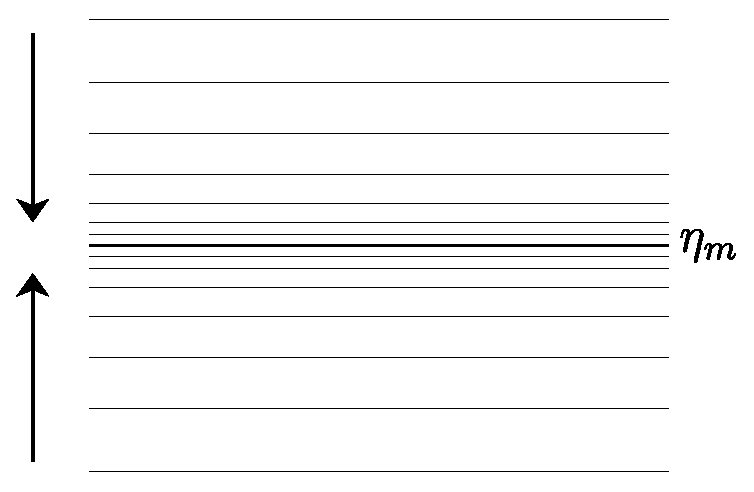
\includegraphics[width=80mm]{./Imagenes/densidad-eta-linea}}
					\hspace{1cm}
					\subfigure[Efecto de atracción al punto $(\xi_{n}, \eta_{n})$]{\label{fig:densidad-eta-punto}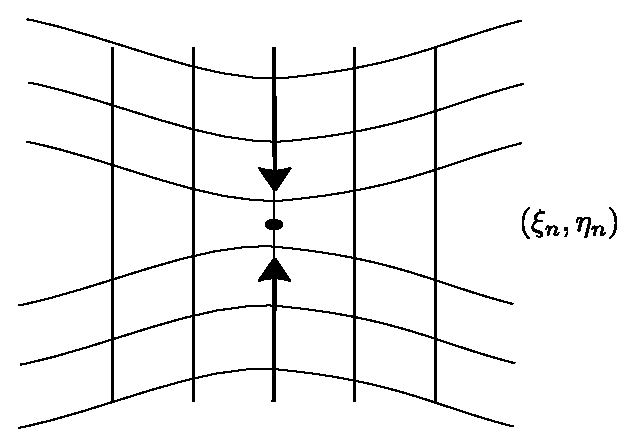
\includegraphics[width=80mm]{./Imagenes/densidad-eta-punto}}
					\caption[Efecto de atracción por función $Q(\xi,\eta)$]{Efecto de atracción en el eje $\eta$ por la función $Q(\xi, \eta)$}
					\label{fig:densidad-eta}
				\end{figure}
			
			\subsection{Algoritmos de solución}
				\paragraph*{}
					Existen en general, dos métodos de solción de sistemas de ecuaciones algebráicas lineales simultáneas: métodos directos y métodos iterativos.
				
				\paragraph*{}
					Dentro de los métodos directos podemos encontrar los métodos de Cramer y de Gauss. La principal desventaja que presentan estos metodos es el gran número de opraciones aritméticas necesarias para obtener una solución del sistema. Desde el punto de vista computacional otras desventajas que presentan son el uso de memoria y cierta dificultad para ser programados. Los métodos iterativos son simples y fáciles de programar, por lo que se presentan como una mejor herramienta para llevar a cabo la solcuión del sistema. La idea de estos métodos, tal y como su nombre lo indica, es obtener la solución mediante un proceso iterativo, por lo general se asume una primera solución y con dichos valores propuestos se calculan nuevos valores de las incógnitas, con base en lo nuevos valores calculados se obtienen nuevos valores. Este proceso se repite hasta satisfacer el criterio de convergencia establecido.
			
			\subsection{Métodos iterativos: Jacobi, Gauss-Seidel, SOR}
				\paragraph*{}
					Para resolver una ecuación matricial de la forma $Au = d$ para el vector $u$ de dimensiones $n \times 1$ suelen utilizarse métodos iterativos. Se pueden escribir las ecuaciones para cada término del vector $u$ (asumiendo que ningún elemento de la diagonal principal de la matriz es igual a $0$) de la siguiente manera
					\begin{subequations}
						\begin{equation*}
							u_{1} = \frac{1}{a_{11}} \left[ d_{1} - \left( a_{12}u_{2} + a_{13}u_{3} + \dotsb + a_{1n}u_{n} \right) \right]
						\end{equation*}
						\begin{equation*}
							u_{2} = \frac{1}{a_{22}} \left[ d_{2} - \left( a_{21}u_{1} + a_{23}u_{3} + \dotsb + a_{2n}u_{n} \right) \right]
						\end{equation*}
						\begin{equation*}
							\dotsb
						\end{equation*}
						\begin{equation*}
							u_{n} = \frac{1}{a_{nn}} \left[ d_{n} - \left( a_{n1}u_{1} + a_{n2}u_{2} + \dotsb + a_{n\left( n-1 \right)}u_{n-1} \right) \right]
						\end{equation*}
					\end{subequations}
				\paragraph*{}
					A partir de estas ecuaciones se derivan varios esquemas iterativos, dada una solución inicial $u_{i}^{(1)}, i = 1, 2, \dotsc, n$. El primero de ellos es el método de Jacobi, en éste, la variable dependiente se calcula usando los datos previamente obtenidos, quedando sus ecuaciones cómo
					\begin{subequations}
						\begin{equation*}
							u_{1}^{k+1} = \frac{1}{a_{11}} \left[ d_{1} - \left( a_{12}u_{2}^{k} + a_{13}u_{3}^{k} + \dotsb + a_{1n}u_{n}^k \right) \right]
						\end{equation*}
						\begin{equation*}
						u_{2}^{k+1} = \frac{1}{a_{22}} \left[ d_{2} - \left( a_{21}u_{1}^{k} + a_{23}u_{3}^{k} + \dotsb + a_{2n}u_{n}^{k} \right) \right]
						\end{equation*}
						\begin{equation*}
						\dotsb
						\end{equation*}
					\end{subequations}
					\begin{equation}
						u_{n}^{k+1} = \frac{1}{a_{nn}} \left[ d_{n} - \left( a_{n1}u_{1}^{k} + a_{n2}u_{2}^{k} + \dotsb + a_{n\left( n-1 \right)}u_{n-1}^{k} \right) \right]
						\label{ec-jacobi}
					\end{equation}
					
				\paragraph*{}
					La ecuación \ref{ec-jacobi} es la ecuación constitutiva del método iterativo de Jacobi, en ella $k$ representa los valores previamente calculados, es decir, obtenidos de la iteración anterior o de la solución inicial, según sea el caso. El superíndice $k+1$ indica el valor obtenido en la iteración actual.
				
				\paragraph*{}
					El siguiente método que puede desarrollarse es el método de Gauss-Seidel, el cual utiliza los valores calculados en la iteración actual para calcular los siguientes valores de la variable dependiente. Sus ecuaciones se escriben como
					\begin{subequations}
						\begin{equation*}
						u_{1}^{k+1} = \frac{1}{a_{11}} \left[ d_{1} - \left( a_{12}u_{2}^{k} + a_{13}u_{3}^{k} + \dotsb + a_{1n}u_{n}^k \right) \right]
						\end{equation*}
						\begin{equation*}
						u_{2}^{k+1} = \frac{1}{a_{22}} \left[ d_{2} - \left( a_{21}u_{1}^{k+1} + a_{23}u_{3}^{k} + \dotsb + a_{2n}u_{n}^{k} \right) \right]
						\end{equation*}
						\begin{equation*}
						\dotsb
						\end{equation*}
					\end{subequations}
					\begin{equation}
						u_{n}^{k+1} = \frac{1}{a_{nn}} \left[ d_{n} - \left( a_{n1}u_{1}^{k+1} + a_{n2}u_{2}^{k+1} + \dotsb + a_{n\left( n-1 \right)}u_{n-1}^{k+1} \right) \right]
						\label{ec-GS}
					\end{equation}
					en este método se calcula un nuevo valor $u_{1}^{k+1}$ con los valores de la iteración anterior, dicho valor luego es ocupado para el cálculo de $u_{2}^{k+1}$, ambos términos son utilizados para obtener $u_{3}^{k+1}$ y el proceso continúa de la misma manera hasta llegar a la última ecuación. Es decir, el método de Gauss-Seidel implica el uso inmediato de los valores $u_{i}^{k+1}$ tan pronto como están disponibles lo que da como resultado un uso menor de memoria en el ordenador, además de satisfacer el criterio de convergencia en menos iteraciones comparado con el método de Jacobi. La ecuación \ref{ec-GS} puede escribirse de la siguiente manera
					\begin{align}
						&\begin{aligned}
							u_{i}^{k+1} =& \frac{1}{a_{ii}} \left[ d_{i} - \sum_{j=1}^{i-1} a_{ij}u_{j}^{k+1}  - \sum_{j = i + 1}^{n} a_{ij}u_{j}^{k} \right], &i = 1, 2, \dotsc, n
						\end{aligned}
						\label{ec-GS-2}
					\end{align}
				
				\paragraph*{}
					Si durante el proceso de solución se percibe una tendencia en los valores calculados se puede utilizar la dirección de cambio para extrapolar para la siguiente iteración y por lo tanto, acelerar el proceso de solución. A este procedimiento se le conoce como método SOR (Succesive Over-Relaxation o  Sobre-relajación sucesiva). Este método introduce un parámetro extra $\omega$ conocido como parámetro de aceleración, el cual puede acelerar la convergencia. Dicho método está representado por
					\begin{align}
						&\begin{aligned}
							u_{i}^{k+1} =& u_{i}^{k} + \frac{\omega}{a_{ii}} \left[ d_{i} - \sum_{j = 1}^{i - 1}a_{ij}u_{j}^{k+1} - a_{ii}u_{i}^{k} - \sum_{j = i+1}^{n} a_{ij}u_{j}^{k} \right]
							\\ \\
							=& \frac{\omega}{a_{ii}} \left[ d_{i} - \sum_{j = 1}^{i - 1} a_{ij}u_{j}^{k+1} - \sum_{j = i+1}^{n} a_{ij}u_j ^{k}\right] + \left( 1 - \omega \right) u_{i}^{k}, &i = 1, 2, \dotsc, n
						\end{aligned}
					\end{align}
				
				\paragraph*{}
					Cuando $\omega = 1$ el método SOR se convierte en el método de Gauss-Seidel. Si $1 < \omega < 2$ se está trabajando con sobre-relajación, mientras que al utilizar un valor $0 < \omega < 1$ se lleva a cabo una bajo-relajación.
		
		\section{Generación de mallas mediante EDP hiperbólicas}
		\paragraph*{}
			La generación de mallas mediante EDP elípticas puede ser demasiado costosa en términos de tiempo de cómputo, así como en el uso de memoria en el ordenador. Esto se debe a que dicho esquema intenta hacer coincidir un sistema de coordenadas curvilíneo a cuatro curvas de frontera, seis en mallas tridimensionales. De aquí surge un nuevo enfoque, en el cual solo se requiere iniciar la solución con una sola frontera e ir avanzando hacia afuera en el dominio físico usando EDP hiperbólicas. \cite{farrashkhalvat}
		
		\paragraph*{}
			Con este propósito se toma en cuenta el trabajo publicado por Steger y Chausse \cite{Hyperbolic-steger1980generation} para la generación de mallas bidimensionales ortogonales y con control del área de celda. Se inicia el proceso con una frontera única en la que se considera que $\eta = 0$. Se propone tambien un sistema de ecuaciones de primer orden para las coordenadas $x, y$ como funciones de $\xi, \eta$:
			\begin{subequations}
				\begin{equation}
					g_{12} = g_1  \cdot g_2 = x_{\xi} x_{\eta} + y_{\xi} y_{\eta} = 0
				\end{equation}
				\begin{equation}
					\abs{g_1 \times g_2} = x_\xi y_\eta - x_\eta y_\xi = F
				\end{equation}
				
				\label{ec-hyper-base}
			\end{subequations}
		
		\paragraph*{}
			La primera ecuación dota a la malla de ortogonalidad, mientras que la segunda tiene el término $F$ como una medida del área de la celda (si el producto $\delta\xi\delta\eta$ es el mismo para cada celda). Se puede trabajar utilizando $F$ como una función de $\xi, \eta$, lo que permitiría incrementar la densidad de la malla cerca de la frontera donde $\eta = 0$ haciendo que $F$ tenga un valor pequeño en dicha zona. De las ecuaciones \ref{ec-hyper-base}:
			\begin{subequations}
				\begin{equation}
					x_\eta = - \frac{F}{ x_\xi ^ 2 + y_\xi ^ 2 } y_\xi
				\end{equation}
				\begin{equation}
					y_\eta = \frac{F}{ x_\xi ^ 2 + y_\xi ^ 2 } x_\xi
				\end{equation}
			\end{subequations}
		
		\paragraph*{}
			Antes de proceder a la solución del sistema de las ecuaciones \ref{ec-hyper-base} se deben tomar en cuenta algunas consideraciones. En primera instancia debe tenerse en cuenta que el sistema es un sistema no lineal por lo que un proceso de linearización debe llevarse a cabo, una segunda consideración es que al ser un sistema de ecuaciones hiperbólicas de debe llevar a cabo el proceso de solución mediante un proceso de marcha, en este trabajo la marcha se realizará en la dirección del eje $\eta$. Tercera, para un sistema de ecuaciones hiperbólicas se debe especificar una condicion inicial así como un condición de frontera y por último, con el objetivo de evitar la presencia de oscilaciones, se puede agregar un término de``damping'' al lado derecho de las ecuaciones.
			
		\paragraph*{}
			Para el proceso de linearización, se utilizará el esquema iterativo de Newton, el cual especifica que un termino no lineal es aproximado mediante
			\begin{equation}
				AB = A^{k + 1} B^{k} + B^{k + 1} A^{k} - A^{k} B^{k}
			\end{equation}
			donde el superíndice $k$ representa el estado previo conocido. A partir de este punto el superíndice $k + 1$, el cual representa el nivel actual a obtener, será eliminado de las ecuaciones, y se entiende que todos los términos sin superíndice pertenecen al nivel actual $k + 1$. Por lo tanto, el sistema de ecuaciones hiperbólicas es expresado en su forma lineal como:
			\begin{subequations}
				\begin{equation}
					x_{\xi} x_{\eta}^{k} + x_{\xi}^{k} x_{\eta} - x_{\xi}^{k} x_{\eta}^{k} + y_{\xi} y_{\eta}^{k} + y_{\xi}^{k} y_{\eta} - y_{\xi}^{k} y_{\eta}^{k} = 0
				\end{equation}
				\begin{equation}
					x_{\xi} y_{\eta}^{k} + x_{\xi}^{k} y_{\eta} - x_{\xi}^{k} y_{\eta}^{k} - x_{\eta} y_{\xi}^{k} - x_{\eta}^{k} y_{\xi} + x_{\eta}^{k} y_{\xi}^{k} = F
				\end{equation}
				\label{ec-hyper-linear}
			\end{subequations}
		
		\paragraph*{}
			Aplicando el concepto de las ecuaciones \ref{ec-hyper-base} a las ecuaciones \ref{ec-hyper-linear} podemos simplificar las últimas, quedando como
			\begin{subequations}
				\begin{equation}
					x_{\xi} x_{\eta}^{k} + x_{\xi}^{k} x_{\eta} + y_{\xi} y_{\eta}^{k} + y_{\xi}^{k} y_{\eta} = 0
				\end{equation}
				\begin{equation}
					x_{\xi} y_{\eta}^{k} + x_{\xi}^{k} y_{\eta} - x_{\eta} y_{\xi}^{k} - x_{\eta}^{k} y_{\xi} = F + F^{k}
				\end{equation}
				\label{ec-hyper-reducida}
			\end{subequations}
		
		\paragraph*{}
			Este sistema de ecuaciones puede escribirse de forma compacta como
			\begin{equation}
				\left[A \right] R_{\xi} + \left[ B \right] R_{\eta} = H
				\label{ec-hyper-compacta}
			\end{equation}
			donde:
			\begin{align*}
				R = \begin{bmatrix}
				 x \\ \\
				 y
				\end{bmatrix}&&
				A = \begin{bmatrix}
					x_{\eta}^{k} & y_{\eta}^{k} \\ \\
					y_{\eta}^{k} & -x_{\eta}^{k}
				\end{bmatrix}&&
				B = \begin{bmatrix}
					x_{\xi}^{k} & y_{\xi}^{k} \\ \\
					-y_{\xi}^{k} & x_{\xi}^{k}
				\end{bmatrix}&&
				H = \begin{bmatrix}
					0 \\ \\
					F + F^{k}
				\end{bmatrix}
			\end{align*}
		
		\paragraph*{}
			Por definición, el sistema de ecuaciones descrito por la ecuación \ref{ec-hyper-compacta} es hiperbólico los eigenvalores de $\left[ B \right]^{-1} \left[ A \right]$ son reales. Se observa que\\
			\begin{equation*}
				\left[ B \right] = \frac{1}{DN}\begin{bmatrix}
					x_{\xi}^{k} & -y_{\xi}^{k} \\ \\
					y_{\xi}^{k} & x_{\xi}^{k}
				\end{bmatrix}
			\end{equation*}
			por lo tanto
			\begin{equation*}
				\left[ C \right] = \left[ B \right]^{-1} \left[ A \right] = \begin{bmatrix}
					x_{\xi}^{k} x_{\eta}^{k} - y_{\xi}^{k} y_{\eta}^{k} &
					x_{\xi}^{k} y_{\eta}^{k} + x_{\eta}^{k} y_{\xi}^{k} \\ \\
					x_{\xi}^{k} y_{\eta}^{k} + x_{\eta}^{k} y_{\xi}^{k} &
					- \left( x_{\xi}^{k} x_{\eta}^{k} - y_{\xi}^{k} y_{\eta}^{k} \right)
				\end{bmatrix}
			\end{equation*}
			donde
			\begin{equation*}
				DN = \left( x_{\xi}^{k} \right)^2 + \left( y_{\xi}^{k} \right)^2
			\end{equation*}
		
		\paragraph*{}
			Los eigenvalores de $\left[ C \right]$ son
			\begin{equation*}
				\lambda_{1, 2} = \pm \left[ \frac{\left(x_{\eta}^{k} \right)^2 + \left( y_{\eta}^{k} \right)^2} {DN} \right]
			\end{equation*}
			los cuales cumplen con la condición de ser siempre reales (para un sistema hiperbólico) siempre que
			\begin{equation*}
			DN = \left( x_{\xi}^{k} \right)^2 + \left( y_{\xi}^{k} \right)^2 \neq 0
			\end{equation*}
		 \paragraph*{}
			 Para obtener un sistema de ecuaciones algebráico, debemos aplicar el método de diferencias finitas. Para la sustitución de las derivadas parciales respecto al eje $\xi$ se utiliza una aproximación central de segundo order y para el caso de las derivadas parciales respecto al eje $\eta$ se hará uso de aproximaciones de primer orden tipo ``forward'', resultando la ecuación en
			 \begin{equation}
				 \left[ A \right] \frac{R_{i + 1, j} - R_{i - 1, j}}{2 \Delta \xi} + \left[ B \right] \frac{R_{i, j} - R_{i, j - 1}}{\Delta \eta} = \left[ H \right]_{i, j}
			 \end{equation}
			 que al ser multiplicada por la matriz $\left[ B \right]^{-1}$ y reacomodada queda cómo
			 \begin{equation}
				 \frac{R_{i, j} - R_{i, j-1} }{\Delta \eta} + \left[ B \right]^{-1} \left[ A \right] \frac{R_{i + 1, j} - R_{i - 1, j} }{2 \Delta \xi} = \left[ B \right]^{-1} H_{i, j}
			 \end{equation}
			 en donde las matrices $A$ y $B$ son evaluadas en la línea $(j - 1)$. Esta ecuación se reacomoda y se le asignan nuevos términos, con el propósito de compactar a la misma, dando como resultado
			 \begin{equation}
				 \left[ AA \right] R_{i - 1, j} + \left[ BB \right] R_{i, j} + \left[ CC \right] R_{i + 1, j} = \left[ DD \right]_{i, j}
				 \label{ec-hyper-final}
			 \end{equation}
			 donde
			 \begin{subequations}
			 	\begin{equation*}
				 	\left[ AA \right] = - \frac{1}{2} \left[ C \right]_{i, j - 1}
			 	\end{equation*}
				\begin{equation*}
					\left[ BB \right] = \left[ I \right]
				\end{equation*}
				\begin{equation*}
					\left[ CC \right] = \frac{1}{2} \left[ C \right]_{i, j - 1}
				\end{equation*} 
			 \end{subequations}
		 una vez que se ha desarrollado la ecuación \ref{ec-hyper-final} para todas las instancias existentes a lo largo de $i$ para un mismo nivel $j$, se obtiene un sistema de bloque tridiagonal
		 \begin{equation}
			 \begin{bmatrix}
				 \left[ BB \right]_2 & \left[ CC \right]_2 & & & & \\
				 \left[AA\right]_3 & \left[BB\right]_3 & \left[CC\right]_3 & & & \\
				 & \ddots & \ddots &  \ddots & & \\
				 & & \ddots & \ddots & \ddots & & \\
				 & & & \left[AA\right]_{m-2} & \left[BB\right]_{m-2} & \left[CC\right]_{m-2}\\
				 & & & & \left[AA\right]_{m-1} & \left[BB\right]_{m-1}
			 \end{bmatrix}
			 \begin{bmatrix}
				 R_{2}\\
				 R_{3}\\
				 \vdots\\
				 \vdots\\
				 R_{m-2}\\
				 R_{m-1}
			 \end{bmatrix}
			 = \begin{bmatrix}
				 \left[DD\right]_2\\
				 \left[DD\right]_3\\
				 \vdots\\
				 \vdots\\
				 \left[DD\right]_{m-2}\\
				 \left[DD\right]_{m-1}
			 \end{bmatrix}
		 \end{equation}
		 los términos $\left[DD\right]_2$ y $\left[DD\right]_{m - 1}$ son afectados por las condiciones de frontera de la siguiente manera
		 \begin{subequations}
		 	\begin{equation*}
			 	\left[DD\right]_2 = \left[DD\right]_2 - \left[AA\right]_2 R_1
		 	\end{equation*}
		 	\begin{equation*}
			 	\left[DD\right]_{m - 1} = \left[DD\right]_{m - 1} - \left[CC\right]_{m - 1} R_{m}
		 	\end{equation*}
		 \end{subequations}
		
	\paragraph*{}
		Este sistema de ecuaciones se resuelve avanzando en dirección del eje $\eta$, siempre y cuando la distribución de punto en la superficie y en las fronteras sea proporcionada.
		
	\paragraph*{}
		Los puntos en las fronteras deben ser libres de flotar, es decir, deben calcularse al final de cada iteración. Esto se logra aplicando la condición de ortogonalidad a las fronteras $i = 1$ e $i = m$ para actualizar dichos puntos.
	
	\subsection{Algoritmo de solución}
	\paragraph*{}
		En el presente proyecto se lleva a cabo la solución del sistema obtenido en la sección anterior mediante el método propuesto por Hoffman\cite{hoffmann2000computational}.
	
	\paragraph*{}
		Un sistema de ecuaciones diferenciales parciales es aproximado mediante un sistema de bloque tridiagonal cuando en dicho sistema se involucran tres puntos de la malla en cada nivel. El sistema resultante puede expresarse en su forma general como:
		\begin{equation}
			S \Delta Q = R
			\label{hyper-sol-1}
		\end{equation}
		donde $\Delta Q$ y $R$ con vectores con $m$ componentes, y a su vez, $S$ representa el bloque tridiagonal
		\begin{equation*}
			S = \begin{bmatrix}
			B_2 & C_2\\
			A_3 & B_2 & C_3\\
			& A_4 & B_4 & C_4\\
			& & \ddots & \ddots & \ddots\\
			& & & A_{m-2} & B_{m-2} & C_{m-2}\\
			& & & & A_{m-1} & B_{m-1}
			\end{bmatrix}
		\end{equation*}
		donde $A_i, B_i$ y $C_i$ son matrices de orden $m$.
		
	\paragraph*{}
		Para poder continuar con la obtención de un esquema de solución, habrá que considerar la siguiente factorización
		\begin{equation}
			S = LU = \begin{bmatrix}
				\alpha_2\\
				A_3 & \alpha_3 \\
				& A_4 & \alpha_4\\
				& & \ddots & \ddots\\
				& & & A_{m-2} & \alpha_{m-2}\\
				& & & & A_{m-1} & \alpha_{m-1}
			\end{bmatrix}
			\begin{bmatrix}
				I & \beta_2\\
				& I & \beta_3\\
				& & I & \beta_4\\
				& & & \ddots & \ddots\\
				& & & & I & \beta_{m-2}\\
				& & & & & I\\
			\end{bmatrix}
		\end{equation}
		donde $I$ es la matriz identidad de orden $m$ y las matrices cuadradas $\alpha_i$ y $\beta_i$ se determinan mediante
		\begin{align}
			\alpha_2 = B_2 && y && \beta_2 = B_{2}^{-1} C_2
		\end{align}
		\begin{align}
			\alpha_i = B_i - A_i \beta_{i-1} &&&& i = 3, 4, \dots, m-1
		\end{align}
		y
		\begin{align}
			\beta_i = \alpha_{i}^{-1} C_i &&&& i = 3, 4, \dots, m-2
		\end{align}
		
	\paragraph*{}
		Ahora, el sistema dado por la ecuación \ref{hyper-sol-1} es equivalente a
		\begin{equation}
			LY = R
			\label{hyper-sol-2}
		\end{equation}
		donde
		\begin{equation}
			Y = U \Delta Q
			\label{hyper-sol-3}
		\end{equation}
	
	\paragraph*{}
		La ecuación \ref{hyper-sol-2} al desarrollarse queda de la siguiente manera
		\begin{equation}
			\begin{bmatrix}
				\alpha_2\\
				A_3 & \alpha_3\\
				& A_4 & \alpha_4\\
				& & \ddots & \ddots\\
				& & & A_{m-1} & \alpha_{m-1}
			\end{bmatrix}
			\begin{bmatrix}
				Y_2\\
				Y_3\\
				Y_4\\
				\vdots\\
				Y_{m-1}
			\end{bmatrix}
			=
			\begin{bmatrix}
				R_2\\
				R_3\\
				R_4\\
				\vdots\\
				R_{m-1}
			\end{bmatrix}
		\end{equation}
		donde
		\begin{equation}
			Y_2 = \alpha_{2}^{-1} R_2
		\end{equation}
		y
		\begin{align}
			Y_i = \alpha_{i}^{-1} \left( R_i - A_i Y_{i-1} \right) &&&& i = 3, 4, \dots, m-1
		\end{align}
		
	\paragraph*{}
		La ecuación \ref{hyper-sol-3} se desarrolla como
		\begin{equation}
			\begin{bmatrix}
				I & \beta_2\\
				& I & \beta_3\\
				& & I & \beta_4\\
				& & & \ddots & \ddots\\
				& & & & I & \beta_{m-2}\\
				& & & & & I
			\end{bmatrix}
			\begin{bmatrix}
				\Delta Q_2\\
				\Delta Q_3\\
				\Delta Q_4\\
				\vdots\\
				\Delta Q_{m-2}\\
				\Delta Q_{m-1}
			\end{bmatrix}
			=
			\begin{bmatrix}
				Y_2\\
				Y_3\\
				Y_4\\
				\vdots\\
				Y_{m-2}\\
				Y_{m-1}
			\end{bmatrix}
		\end{equation}
		en donde
		\begin{equation}
			\Delta Q_{m-1} = Y_{m-1}
		\end{equation}
		y
		\begin{align}
			\Delta Q_i = Y_i - \beta_i \Delta Q_{i+1} &&&& i = m-1, m-2, \dots, 3, 2
		\end{align}
		
			
				
	%
	%
	%
	%
	%
	
	%
	%
	%
	%
	%
\chapter{Desarrollo Práctico}
	\paragraph*{}
		Los códigos de este trabajo fueron implementados en lenguaje Python 3, utilizando el paradigma de programación orientada a objetos, en éste los datos son trabajados como objetos con atributos y métodos pertenecientes a una clase, y que pueden ser heredados y aplicados a objetos o instancias de alguna subclase. Un objeto  es la representación en un programa de un concepto y contiene toda la información necesaria para abstraerlo, como son los datos que describen sus atributos y operaciones que pueden realizarse dobre los mismos.  En otras palabras un objetos es la relación que existe entre un conjunto de variables y métodos.
	
	\paragraph*{}
		Se dice que todos las instancias (objetos) de un mismo tipo, son pertenecientes a una misma clase. Una de las características más importantes de la programación orientada a objetos es la herencia, la cual permite la definición de nuevas clases a partir de una ``superclase'' ya existente, las cuales se conocen como ``subclases''. Una subclase hereda todo el comportamiento de su superclase, pero se puede introducir además características propias.
		
	\paragraph*{}
		En el presente trabajo se implementaron dos superclases: ``airfoil'' y ``mesh'', cada una con sus respectivas subclases.
		La clase airfoil se desarrolló para la creación de perfiles alares a partir de una archivo de texto que contenga la nube de puntos del perfil deseado, como dato de entrada se requiere el nombre del archivo texto y la dimensión en metros de la cuerda. Esta clase tiene una subclase ``NACA4'' la cual genera perfiles de la serie de 4 dígitos de perfiles aerodinámicos de la NACA. La creación del perfil se hace a partir de la ecuación constitutiva de la serie. Como datos de entrada se requieren los valores de m (combudara máxima), p (posición de la combadura máxima), t (espesor máximo) y c (cuerda). La subclase NACA4 tiene dos métodos para la creación del perfil, el primero de ellos, el método ``create\textunderscore linear'' crea la nube de puntos con una distribución equidistante de los puntos en dirección del eje $x$. El segundo método, llamado ``create\textunderscore sin''genera a partir de una función senoidal una nube de punto que permite que haya mayor densidad de nodos tanto en el borde de ataque como en el borde de salida del perfil.
			 
			 
				
			
		 
		
		
		
		
	%
	%
	%
	%
	%
	
	%
	%
	%
	%
	% Referencias Bibliográicas %
	\cleardoublepage
	\phantomsection % corrige error de hipervinculos que manda a la seccion previa
	\addcontentsline{toc}{chapter}{Referencias}
	\bibliography{referencias.bib}
	\bibliographystyle{unsrt}
	
	
	
	

\end{document}